\documentclass[a4paper]{report}
\usepackage[utf8]{inputenc}
\usepackage[T1]{fontenc}
\usepackage{RJournal}
\usepackage{amsmath,amssymb,array}
\usepackage{booktabs}

%% load any required packages FOLLOWING this line
\usepackage{thumbpdf,lmodern}
\usepackage{soul}
\usepackage{framed}
\usepackage{subfig}

\newcommand{\class}[1]{`\code{#1}'}
\newcommand{\fct}[1]{\code{#1()}}
\newcommand{\btheta}{\boldsymbol{\theta}}
\newcommand{\balpha}{\boldsymbol{\alpha}}
\newcommand{\bmu}{\boldsymbol{\mu}}
\newcommand{\bSigma}{\boldsymbol{\Sigma}}
\newcommand{\bbeta}{\boldsymbol{\beta}}
\newcommand{\bnu}{\boldsymbol{\nu}}
\newcommand{\bx}{\boldsymbol{x}}
\newcommand{\bw}{\boldsymbol{w}}
\newcommand{\bbf}{\boldsymbol{f}}
\newcommand{\blambda}{\boldsymbol{\lambda}}
\newcommand{\bg}{\boldsymbol{g}}
\newcommand{\pos}{\mbox{\textbf{pos}}}
\newcommand{\posi}{\mbox{\textbf{pos}}^{imp}}
\newcommand{\posc}{\mbox{\textbf{pos}}^{col}}
\DeclareMathOperator{\tr}{tr}
%%\DeclareMathOperator{\var}{\mbox{Var}}
\DeclareMathOperator{\argmin}{argmin}
\newcommand{\diag}{\mbox{\textbf{diag}}}


\begin{document}

%% do not edit, for illustration only
\sectionhead{Contributed research article}
\volume{14}
\volnumber{3}
\year{2022}
\month{September}
\setcounter{page}{20}

%% replace RJtemplate with your article
\begin{article}
  %\input{ICAODV1}
    % !TeX root = RJwrapper.tex
\title{ICAOD: An R Package for Finding Optimal designs for Nonlinear Statistical Models by Imperialist Competitive Algorithm}
\author{by Ehsan Masoudi, Heinz Holling, Weng Kee Wong and Seongho Kim}

\maketitle

\abstract{
  Optimal design ideas  are increasingly used in different disciplines to rein in experimental costs.
  Given a nonlinear statistical model and a design criterion, optimal designs determine the number of experimental points to observe the responses,  the design points and the  number of replications at each design point.
  Currently, there are very few free and effective computing tools for finding different types of optimal designs for a general nonlinear model, especially when the criterion is not differentiable.
  We introduce an  R package  \CRANpkg{ICAOD}  to find various types of optimal designs and they include   locally, minimax and Bayesian optimal designs for different nonlinear statistical models.  Our main computational tool  is a novel metaheuristic algorithm called imperialist competitive algorithm (ICA) and   inspired by  socio-political behavior of humans and colonialism.  We demonstrate its capability and effectiveness using several applications. The package also includes several theory-based tools to assess  optimality of a generated design  when the criterion is a convex function of the design.
}

\section{Introduction}\label{sec:intro}
Optimal designs have been extensively applied in many research studies to reduce the cost of experimentation.   For instance,
\citet{holling2013introduction} provided examples  in psychology and \citet{dette2010optimal} gave examples in dose-response studies. Further applications of optimal designs in engineering and epidemiology are described in \citet{bergerwong2009},  which also contains applications of optimal design ideas  in other disciplines.
Given a statistical model and an optimality criterion, optimal designs determine the  optimal number of design points required,  their locations  to observe the responses and the  number of replications required at each location.  The
optimality criterion should accurately reflect the objective of the study to the extent possible and is usually formulated as a scalar function of  the Fisher information matrix (FIM) that measures the worth of the design \citep{lehmann1998theory}.
For example, if the objective of a study is to estimate the model parameters as accurately as possible, $ D$-optimality is often used.  Such an optimal design maximizes the determinant of the FIM and is called $D$-optimal.  When errors are independent and normally distributed, $D$-optimal designs minimize the volume of the confidence ellipsoid of the model parameters by minimizing the generalized variance, i.e.,  the determinant of the variance-covariance matrix \citep{abdelbasit1983}.

For nonlinear models, the FIM  depends on the unknown model parameters to be estimated and so the design criterion cannot be directly optimized.  There are
different approaches   to deal with this parameter dependency: a) {\it locally optimal designs:} These are   found by replacing the  unknown parameters with some estimates obtained from a pilot or previous study \citep{chernoff1953}.
Locally optimal  designs usually become inefficient when the replaced estimates  are far  from their true unknown values.
b) {\it minimax optimal designs:} They minimize the maximum inefficiency over a user-selected  parameter space \citep{sitter1992}. The optimal designs are conservative in   that they protect the experiment from the worst case scenario that may happen from a poor choice of parameter values over  a user-specified space of plausible values for the unknown parameters.  Finding minimax optimal  designs is  complicated  because it involves solving  multi-level nested optimization problems  and the objective function (minimax criterion) is not differentiable. c) {\it Bayesian optimal designs:}  These optimal designs
are found by optimizing an  optimality criterion averaged over a user-specified (continuous) prior distribution for the unknown parameters  \citep{chaloner1989, chaloner1995, Atkinson1996}.
Strictly speaking, the latter are not fully Bayesian because they do not involve computing a posterior distribution.
Instead, they borrow the concept of having prior distributions to find robust designs for the frequentists \citep{grasshoff2012optimal, burkner2019optimal}. Accordingly,  they are  sometimes referred to as ``pseudo'' Bayesian  designs \citep{firth1997bayesian}.  In the optimal design literature,  Bayesian optimal designs found under a discrete prior distribution    are  usually referred to as {\it robust } or {\it optimum-on-average} designs  \citep{fedorov2012model}.
For an overview of optimal designs for nonlinear models, see \citet{fedorov2013optimal}.

There are several software packages to  create and analyze  design of experiment (DoE) for different purposes.  For a review on statistical R packages in design of experiments, see  \url{https://cran.r-project.org/web/views/ExperimentalDesign.html}.  Only a few of them are able to  find different types of optimal designs   to deal with the parameter dependency for various nonlinear models.
To the best of our knowledge, none of the available software packages, commercial or otherwise, provides an option to  find  minimax optimal designs for nonlinear models.
For example,  the R package \CRANpkg{LDOD} \citep{masoudi2013}   finds locally $D-$optimal {\it approximate} designs for a large class of nonlinear models
and the \CRANpkg{acebayes} R package \citep{overstall2017acebayes} determines a more general class of fully  Bayesian {\it exact} designs  using  the approximate coordinate exchange algorithm \citep{overstall2017bayesian}. Likewise, the recently available
\CRANpkg{VNM} R package  finds multiple-objective locally optimal designs for a specific model, i.e., the four-parameter Hill model commonly used in dose-response studies \citep{VNM-JSS}.
Among the commercial software, JMP\textsuperscript{\textregistered} \citep{jmp13-design}  can also find Bayesian $D-$optimal exact designs for nonlinear models.

This paper introduces the R package \CRANpkg{ICAOD} \citep{ICAOD2020} for finding a variety of  optimal designs for nonlinear models using  a novel metaheuristic algorithm called   {\it imperialist competitive algorithm(ICA)}.
This algorithm  is inspired by  socio-political behavior of humans \citep{ica2007, hosseini2014} and is modified by \citet{masoudi2017} and \citet{masoudi2019} to find optimal designs for nonlinear models.
We believe that this \CRANpkg{ICAOD} package  is the first single self-contained statistical package  that presents  a framework to find   locally, minimax and Bayesian optimal designs for nonlinear models.
Similar to many   popular nature-inspired metaheuristic algorithms, such as particle swarm optimization (PSO) algorithm \citep{Kennedy1995},   ICA  does not have a rigorous  proof of convergence \citep{yang2011metaheuristic}.  When the criterion is a convex function on the set of design measures, equivalence theorems are available  and the \CRANpkg{ICAOD} package includes tools    to confirm optimality of a design.  More generally,  the proximity of any  design to the optimum without knowing the latter can be evaluated in terms of an  efficiency lower bound. In particular, if this bound is unity, this confirms optimality of the design. This feature is  useful to  recognize a case of  pre-mature convergence in optimal design problems.


%Section~\ref{sec:background} 
The next section reviews the statistical setup and theory for finding optimal designs for  nonlinear models.
%Section~\ref{sec:ICA} 
The fourth section describes the imperialist competitive algorithm (ICA) and the fifth section
%Section~\ref{sec:ICAOD-implementation}  
provides  implementation details for  the  \CRANpkg{ICAOD} package.
In  the sixth section, %Section~\ref{sec:examples}, 
we provide two examples to show the functionality of the  \CRANpkg{ICAOD} package. The seventh section %Section~\ref{sec:logsitc-single} 
finds locally and minimax $D-$optimal designs for a logistic model with  application in educational testing and
%Section~\ref{sec:sigmoid} 
The eighth section presents optimum-on-average and Bayesian $D-$optimal designs for a sigmoid Emax model for dose-response studies.
The \CRANpkg{ICAOD} package was first written to find locally  $D-$optimal designs, but it now also finds user-defined optimal designs.  %Section~\ref{sec:new-optimality} 
The ninth section illustrates how to use this feature to find $c-$optimal designs for a two-parameter  logistic model in dose response studies.
%Section~\ref{sec:summary} 
The last section concludes with a summary.


\section{Background and optimal designs}
\label{sec:background}
Let $E(Y)=f(\bx,\btheta)$ be the mean of the response $Y$ at the values of the independent variables $\bx$  defined on   a user-selected   {\it design space} $\chi$, and let  $f$ be a known function, apart from the model parameters $\btheta = (\theta_1,..., \theta_p)^T$.  Throughout we assume that there are resources to take $N$ observations for the study and given an optimality criterion, we want to find the best choices for the levels of the independent variables to observe the outcome $Y$.  There are two types of designs: exact and approximate.An {\it exact}  design $\xi_N$ on $\chi$  is  defined by a set of $k$ distinct  levels $\bx_i$,
\begin{equation}
\label{eq-exact-design}
\xi_N =
  \left\{
    \begin{array}{cccc}
    \bx_1 & \bx_2 & ... & \bx_k\\
    n_1/N & n_2/N & ...& n_k/N
    \end{array}
    \right\},
\end{equation}
where $\bx_j \in \chi$, $n_j$ is  the  number of replications of $\bx_j$ in the observations sample and  $N = \sum_{j=1}^kn_j$.
Here, $x_j, j = 1..., k$  are  referred to as {\it support points} or {\it design points} of $\xi_N$.
Given $N$ and a specific design criterion, an optimal exact design finds the best value of $k$ and the best values of $x_1,\ldots,x_k,n_1,\ldots,n_k$.  Such optimization problems are notoriously difficult and in practice, we find optimal approximate designs instead.  They are probability measure on  $\chi$  are found   independent of the sample size $N$.
An approximate design $\xi$ with $k$ support points has the form
\begin{equation}
\label{eq-approximate-design}
\xi =
  \left\{
    \begin{array}{cccc}
    \bx_1 & \bx_2 & ... & \bx_k\\
    w_1 & w_2 & ...& w_k
    \end{array}
    \right\},
\end{equation}
where $w_j> 0$ is the proportion of observations that is assigned to  $\bx_j$ and $\sum_{j=1}^{k} w_j = 1$.
It is implemented by  first rounding each value of $Nw_i$ to the nearest integer $Nw_i^*$    subject to $Nw_1^*+\ldots+Nw_k^*=N$ and taking $Nw_i*$ observations at $\bx_i,i=1,\ldots,k$.  Some optimal rounding procedures are available in \citet{pukelsheim1992}.
When the design criterion is formulated as a convex function of the FIM, there are algorithms for finding many types of optimal approximate designs and theory to   confirm optimality of an approximate design.  When the design is not optimal, a theory-based efficiency lower bound of the design is available to determine its proximity to the optimum, without knowing the optimum.  For these reasons, we focus on  optimal approximate designs found under a convex functional in the rest of the paper.

To find an approximate design that minimizes a convex design  criterion $\psi$ over the space of all designs on $\chi$.
We have to determine the optimal number of support points, $k$, the optimal support points $\bx_1,\ldots,\bx_k$ and their corresponding $w_1,\ldots,w_k$. For example, if estimating model parameters is of interest,  $D-$optimality, defined by the logarithm of the determinant of the  inverse of the FIM, is a convex functional  over the space of all designs on $\chi$ \citep{fedorov2013optimal, silvey1980} and the design that minimuzes it is  called $D-$optimal. In what follows, we  focus on the $D-$optimality criterion and briefly discuss other  optimality criteria and optimal designs which can be studied similarly.


Assuming  all observation errors are independent and normally distributed  with means $0$ and a constant variance $\var(Y)$,   the  FIM of a generic $k$-point approximate  design $\xi$ is given by
\begin{equation}
\label{eq:FIM}
M(\xi,\btheta) =  \sum_{i=1}^k w_i I(\boldsymbol{x}_i,\btheta),
\end{equation}
where
\begin{equation*}
I(\boldsymbol{x}_i,\btheta) = \frac{1}{\var(Y_i)}\nabla f(\boldsymbol{x}_i,\btheta)\nabla f(\boldsymbol{x}_i,\btheta)^T,
\end{equation*}
and
$\nabla f(\boldsymbol{x}_i,\btheta)^T=\left(
  \frac{\partial f(\boldsymbol{x}_i,\btheta)}{\partial \theta_1},
  \cdots,\frac{\partial f(\boldsymbol{x}_i,\btheta)}{\partial \theta_p}
  \right)$.
Here, $\frac{\partial f(\boldsymbol{x}_i,\btheta)}{\partial \theta_j}$
  denotes the partial derivative of $f$ with respect to $\theta_j$.
The  FIM  is singular if  $k < p$. To avoid singular designs, i.e., designs with singular Fisher information matrices,  we assume  $k\geq p$.


Clearly, the FIM~\eqref{eq:FIM}  depends on the unknown parameters for nonlinear models.
Different  approaches have been proposed to deal with this parameter dependency
based on the type of information available for the unknown parameters. For example, let  $\btheta_0$ be an initial guess for $\btheta$ available from a similar study.
A locally $D-$optimal design $\xi^*_{loc}$  minimizes
\begin{equation}
\label{eq:locally-criterion}
\psi_{loc}(\xi) =   -\log|M(\xi, \btheta_0)|,
\end{equation}
where   $|\cdot|$ denotes  the determinant.  In practice, it is more realistic to assume that the unknown parameters belong to a user-specified parameter space $\Theta$, which  is comprised of all possible values  for $\btheta$. Given $\Theta$, we can find minimax optimal designs that minimize the maximum inefficiency over $\Theta$ and protect the experiment from the worst-case scenario over the parameter space.
A minimax $D-$optimal design $\xi^*_{min}$   is obtained by minimizing
\begin{equation}
\label{eq:minimax-criterion}
\psi_{min}(\xi) =  \max_{\btheta \in \Theta}  -\log|M(\xi, \btheta)|,
\end{equation}
over the space of all designs on $\chi$. The minimax problem~\eqref{eq:minimax-criterion} is a bi-level nested optimization problem with inner and outer optimization problems. Given any arbitrary design, the inner optimization problem is to maximize the $D-$criterion $-\log|M(\xi, \btheta)|$ over $\Theta$ to find the maximum inefficiency  and  the  outer  optimization problem is to  minimize the maximum of the inner problem over  the space of all designs on $\chi$. 
Alternatively,  when a prior distribution $\pi_{\Theta}(\btheta)$  is available for the unknown parameters on $\Theta$, Bayesian optimal designs may also be found: a (pseudo) Bayesian  $D-$optimal design $\xi_{bayes}^*$ minimizes
\begin{equation}
\label{eq:bayesian-criterion}
\psi_{bayes}(\xi) = \int_{\btheta \in \Theta}  -\log|M(\xi, \btheta)| \pi_{\Theta}(\btheta) d\btheta.
\end{equation}
When   $\pi_{\Theta}(\btheta)$ is a discrete prior, the obtained designs are sometimes referred to as  {\it optimum-on-average} or {\it robust}  designs.


One advantage of working with approximate designs is existence of an  equivalence theorem, which can be used to verify the optimality of a given design if the criterion is a convex function on the set of design measures. 
Each convex optimality criterion gives rise to a different equivalence theorem, but they generally have the same form.
For example, a design $\xi_{loc}^*$ is locally $D-$optimal  if and only if the following inequality holds for all $\bx \in \chi$,
\begin{equation}
\label{eq:sensitivity-locally}
c_{loc}(\bx, \xi_{loc}^*) = \tr M^{-1}(\xi_{loc}^*, \btheta_{0})I(\bx, \btheta_{0}) - p \leq 0,
\end{equation}
with equality in~\eqref{eq:sensitivity-locally} at all support points of $\xi_{loc}^*$.
The left hand-side of  inequality~\eqref{eq:sensitivity-locally} is  sometimes called {\it sensitivity function}.
The equivalence theorem for Bayesian $D-$optimality criterion is very similar \citep{kiefer1959,chaloner1989}: a design $\xi_{bayes}^*$ is a Bayesian $D-$optimal design if and only if the following inequality holds for all $\bx \in \chi$,
\begin{equation}
\label{eq:sensitivity-bayesian}
c_{bayes}(\bx, \xi_{bayes}^*) = \int_{\Theta} \mbox{tr} \{ M^{-1}(\xi_{bayes}^*, \btheta)I(\bx, \btheta)\}\pi(\btheta) d\theta-p \leq 0,
\end{equation}
with equality in~\eqref{eq:sensitivity-bayesian} at all support points of $\xi_{bayes}^*$. However, the  equivalence theorem for  a minimax type criterion  takes on a more complicated form because~\eqref{eq:minimax-criterion} is not differentiable. The equivalence theorem states that a design $\xi^*_{min}$ is minimax $D-$optimal among all the designs on $\chi$ if and only if there exists a probability measure $\mu^*$ on
\begin{equation}
\label{eq:A-set}
A(\xi_{min}^*) = \left\{\bnu \in \Theta \mid -\log|M(\xi_{min}^*, \bnu)| = \max_{\btheta \in \Theta} -\log|M(\xi_{min}^*, \btheta)| \right\},
\end{equation}
such that the following inequality holds for all $\bx \in \chi$,
\begin{equation}
\label{eq:sensitivity-minimax}
c_{min}(\bx, \xi_{min}^*) = \int_{A(\xi_{min}^*)} \tr M^{-1}(\xi_{min}^*, \bnu) I(\bx, \bnu)\mu^* d(\bnu)-p \leq 0,
\end{equation}
with equality in~\eqref{eq:sensitivity-minimax} at all support points of $\xi_{min}^*$ \citep{wong1992, fedorov1980convex, king2000, berger2000}.
The set $A(\xi_{min}^*)$ is sometimes called the {\it answering set} of $\xi^*$ and the measure $\mu^*$ is a sub-gradient of the non-differentiable criterion evaluated at $M(\xi_{min}^*,\nu)$.
Understanding the properties of the sub-gradients and how to find them efficiently for the minimax  optimal design problems present a key problem in solving this type of problems.    In particular,  there is no theoretical rule on how to choose the number of points in $A(\xi_{min}^*)$  as support for the measure $\mu^*$ and they would have to be found by trial-and-error. For more details, see \citet{masoudi2017}.
When $\chi$ is one or two dimensional, it is very common to plot the sensitivity function versus $\bx \in \chi$ and  visually inspect whether the graph meets the conditions in the equivalence theorem.  If it does, the generated design is optimal; otherwise it is not optimal.

We measure the efficiency  of one design $\xi_1$ relative to another design $\xi_2$ using their criterion values.
For example, for $D-$optimality~\eqref{eq:locally-criterion}, we use
\begin{equation}
\label{eq:locally-D-efficiency}
\mbox{eff}_{loc} =\left(\frac{|M(\xi_1, \btheta)|}{|M(\xi_2, \btheta)|}\right)^{1/p} =\exp\left(\frac{\psi_{loc}(\xi_2) - \psi_{loc}(\xi_1) }{p}\right).
\end{equation}
The relative $D-$efficiency~\eqref{eq:locally-D-efficiency} may be interpreted in term of sample size; if its value  is $\rho$, then $\xi_1$ requires $1/\rho$ times as many observations to have the same $D-$efficiency as $\xi_2$.
This means that, when $\xi_2$ is an optimal design,  about $(1/\rho-1)100\%$ more number of observations are required for design $\xi_1$ to do as well as the optimal design. Similarly, we define Bayesian and minimax $D-$efficiencies by replacing $\psi_{loc}$ with $\psi_{min}$ and $\psi_{bayes}$, respectively. Standardly, ~\eqref{eq:locally-D-efficiency} becomes the $D-$efficiency of $\xi_1$ when $\xi_2$ is the $D-$optimal design.

When the design criterion is a convex functional, we can use the equivalence theorem to  quantify the proximity of a design $\xi$ to the optimal design without knowing the latter by means of the efficiency lower bound (ELB). For example, for $D-$optimality, we have
\begin{equation}
\label{eq:ELB}
\mbox{ELB} = \frac{p}{p + \max_{\bx \in \chi}c(\bx, \xi)},
\end{equation}
where $c(\bx, \xi)$ is the sensitivity function associated with $D-$optimality. The value of the ratio in ~\eqref{eq:ELB} is between $0$ and $1$, and it is equal to $1$  if and only if the design is optimal. The efficiency bounds are not unique and can be varously derived using somewhat similar arguments, for example, see  \citet{atwood1969optimal} and \citet{pazman1986foundations}.



\section{Imperialist competitive algorithm for finding optimal designs}
\label{sec:ICA}
The imperialist competitive algorithm (ICA) is an evolutionary algorithm inspired from colonialism and socio-political behavior of humans, where developed countries attempt to take over or colonize less-developed countries  to use their resources and  extend their power \citep{ica2007}. Within the optimization framework,  ICA has a population of solutions called {\it countries}. In optimal design problems, each country is the location of the  support  points and the corresponding weights of a design on the space of all possible designs.
ICA divides the population of countries into some sub-populations called {\it empires}. Each empire contains one {\it imperialist} and some {\it colonies}.  The imperialist is the most powerful country within the empire. Here,  the power of a country is defined to be a function of its cost value, i.e., criterion value. This means that, in a minimization problem, countries with smaller cost values are stronger.
In ICA, there are two types of evolutionary moves: a) evolution within  each empire, and, b) evolution among the empires.
In the earlier, the colonies within each empire start to move or be absorbed  toward their relevant imperialist country  in a process  called {\it assimilation} \citep{lin2013imperialist}.
During this process, a colony may reach a  better position than its imperialist.  In this case, the imperialist loses its rank and the colony becomes the new imperialist.
The assimilation  improves searching around the better current solutions and so enhances the exploitation of the algorithm.

The evolution among the empires is achieved by a process called  {\it imperialists competition}. In this process, the most powerful empires receive more chances to take  possession of the colonies of the weakest empires. The competition step in ICA improves  the exploration of the algorithm in a search for the global optimum.
When an empire does not have any colony, it will be eliminated.
ICA continues until it satisfies the stopping rule conditions.
For more details, see \citet{ica2007} and \citet{hosseini2014}.

To apply ICA for an optimal design problem, the user should first provide an initial guess about the number of support point $k (\geq p)$.
In practice, the user can start by $p$ and  increment its value by one  until  the equivalence theorem confirms the optimality of the current best  design, which is the country with the least cost value.
In optimal design problems, the ELB defined by~\eqref{eq:ELB} can  be used to build a stopping rule condition for ICA. For example, the algorithm can be stopped  when the value of the  ELB of the best current design is larger than, say,  $0.95$. Clearly, finding ELB in each iteration increases the CPU time required by the algorithm  as another  optimization problem has to be solved to find maximum of the sensitivity function over $\chi$. This is especially true for minimax and Bayesian type criteria, because  the sensitivity function for the earlier involves solving a bi-level nested optimization problem  and the latter requires approximating  integrals. Therefore, we prefer to calculate  the ELB  periodically, say, after every $100$  iterations, instead of every iteration to save the CPU time.


\section{Implementation of optimal design problems in  ICAOD}
\label{sec:ICAOD-implementation}
Different functions are available to find optimal designs for nonlinear models in \CRANpkg{ICAOD}: a) \fct{locally}: Finds  locally optimal designs,  b) \fct{minimax}: Finds minimax optimal designs , c) \fct{bayes}: Finds Bayesian optimal designs and d) \fct{robust}: Finds optimum-on-average or robust designs.
Throughout this paper, we refer to them as ``OD  functions''.
\CRANpkg{ICAOD} uses the S3 object oriented  system and  works with  an object of class \class{minimax}.  The class \class{minimax} has its own \code{plot},  \code{print} and \code{update} method. The \code{plot} method is used to plot the sensitivity function and also calculate the ELB for the output design. The \code{print} method is to display the brief profile of ICA iterations and the summary of identified optimal designs. The \code{update} method is for executing  the algorithm for more number of iterations.
By default, OD functions are defined to determine $D-$optimal designs. In  the section \samp{User-Specified Optimality Criteria}, %Section~\ref{sec:new-optimality}, 
we demonstrate how  to specify user-defined optimality criteria.
In what follows, the OD functions are explained in detail.


\subsection{Locally optimal designs}\label{sec:locally}
The \fct{locally} function  finds locally optimal designs and  its main  arguments are:
  \begin{example}
locally(formula, predvars, parvars, family = gaussian(), fimfunc = NULL,
        lx, ux, k, iter, ICA.control = list(), sens.control = list(),
        crt_func = NULL, sens_func = NULL,
        inipars)
\end{example}
The arguments in the first three lines of codes are common between the OD functions. Table~\ref{tab:overview-shared-arguments} provides an overview of them.
\begin{table}[t!]
\centering
\begin{tabular}{lp{12cm}}
\hline
Argument          &  Description \\ \hline
\code{formula} & A formula  that is the symbolic description of a nonlinear model.  \\
\code{predvars} & A vector of characters that denote the model predictors in \code{formula}.\\
\code{parvars} & A vector of characters that denote the model parameters in \code{formula}.\\
\code{family} &  The distribution of the model response and the link function. It is the same as the one in \fct{glm}.
The default link function is \fct{gaussian}. \\
\code{fimfunc} & (optional) The Fisher information matrix (R \code{function}).
Required if  users wish  to pass the FIM directly. It  takes a \code{function} with arguments  \code{x} (a vector of design points), \code{w} (a vector of associated weights) and \code{param} (a vector of model parameters). Only one of the \code{formula} and \code{fimfunc} arguments must be given.\\ \hline
\code{k} & The number of design points $k$. \\
\code{lx} & A vector of the lower bounds for the model predictors (design space $\chi$).\\
\code{ux} & A vector of the upper bounds for the model predictors  (design space $\chi$).\\
\code{x} & (optional) A vector of design points $\bx$. if given, only the optimal weights, \code{w},  are sought after.  Required when the design points are pre-specified.\\
\hline
\code{ICA.control}  &  A \code{list} of ICA control parameters. By default, it will be created by  \fct{ICA.control}.\\
\code{iter} & The maximum number of iterations.\\
\hline
\code{sens.control} & Control Parameters of the maximization algorithm, which finds the maximum of the sensitivity function~\eqref{eq:sensitivity-locally},  \eqref{eq:sensitivity-minimax} and \eqref{eq:sensitivity-bayesian} over the design space $\chi$.
The obtained maximum is used to  calculate the ELB of a design.  By default, it will be created by  \fct{sens.control}.
\\
\hline
\code{crt\_func} & (optional) A user-specified criterion  (R \code{function}).\\
\code{sens\_func} &  (optional) A user-specified sensitivity function (R \code{function}). \\
\hline
\end{tabular}
\caption{\label{tab:overview-shared-arguments}
  Overview of the most important  common arguments of the  OD functions.}
\end{table}
The arguments in the first line are required to construct the FIM of the model; \code{inipars} is equivalent to $\btheta_0$ in \eqref{eq:locally-criterion} and defines the vector of initial estimates for the model parameters.


The  \CRANpkg{ICAOD}  package includes a formula interface to specify the model of interest.
For example, assume  the two-parameter logistic model defined by
\begin{equation}
\label{eq:logistic-formula}
f(x, \btheta) = \frac{1}{1 + \exp(-b(x-a))},
\end{equation}
where $\btheta = (a, b)$ is the vector of model parameters and $x$ is the model predictor. To define~\eqref{eq:logistic-formula}  in  \CRANpkg{ICAOD}, we can set  \code{formula = ~1/(1 + exp(-b * (x-a)))}, \code{predvars = "x"}, \code{parvars = c("a", "b")} and  \code{family = "binomial"} (or \code{family = binomial()}).
Alternatively, one may pass the FIM of~\eqref{eq:logistic-formula} as an R \code{function}  via the argument  \code{fimfunc} directly. In this option, the arguments of the defined function must be  a) \code{x}: is a \code{vector} of  $(\bx_1, ..., \bx_k)$ in~\eqref{eq-approximate-design},
b)  \code{w}: is a \code{vector} of  $(w_1, ..., w_k)$ in~\eqref{eq-approximate-design},  and c) \code{param}:  is a  \code{vector} of   $\btheta$ in~\eqref{eq:logistic-formula}.
The output is the FIM of~\eqref{eq:logistic-formula} evaluated at
the given \code{x}, \code{w} and \code{param} as a \code{matrix}.

The argument \code{sens.control} is a list of control parameters for  \fct{nloptr} available in the \CRANpkg{nloptr} package  \citep{johnson2014nlopt}. This function is used here to solve  $\max_{\bx \in \chi}c(\bx, \xi)$ for  computing the ELB~\eqref{eq:ELB}. When not given, it will be created automatically   by the function \code{sens.control}.
We recommend not to change its  default values
as they have been successfully tested for a large number of problems.

The \code{crt\_func} and \code{sens\_func} arguments are used to find a user-defined optimal designs, which are described in
%Section~\ref{sec:new-optimality}.
the section \samp{User-Specified Optimality Criteria}.


\subsection{Minimax optimal designs}
\label{sec:minimax}
The  \fct{minimax} function finds minimax optimal designs and  its main  arguments are:
  \begin{example}
minimax(formula, predvars, parvars, family = gaussian(), fimfunc = NULL,
        lx, ux, k, iter, ICA.control = list(), sens.control = list(),
        crt_func = NULL, sens_func = NULL,
        lp, up, n.grid = 0,
        sens.minimax.control = list(), crt.minimax.control = list())
\end{example}
The first three lines of codes are similar to the ones in \fct{locally} and the  rest of the arguments are used  to evaluate the minimax criterion~\eqref{eq:minimax-criterion} and its sensitivity function~\eqref{eq:sensitivity-minimax} at a given design. Table~\ref{tab:overview-criterion-arguments} presents an overview of the  arguments specifically available in \fct{minimax}.


In  \CRANpkg{ICAOD}, the parameter  space $\Theta$ are  either  continuous or discrete. Note that the lower bound and upper bound of $\Theta$  are specified via the arguments  \code{lp} and \code{up}, respectively. When $\Theta$ is continuous,  \CRANpkg{ICAOD}  uses   \fct{nloptr}  to solve the inner maximization problem  in \eqref{eq:minimax-criterion} over $\Theta$ at a given design.
The default optimization algorithm from \fct{nloptr} is
the DIRECT-L algorithm, which is  a deterministic search algorithm based on the systematic division of the search domain into smaller and smaller hyperrectangles \citep{directL2001}.
For our applications, the most influential tuning parameter of \fct{nloptr}  is  the maximum number of function evaluations denoted by \code{maxeval} (its default value  is $1000$) via the  \code{crt.minimax.control} argument.
The parameter space may also be discretized. In this option,  the total number of grid points is equal to \verb|n.grid^p|. When specified, ICA  evaluates the criterion  at these grid points
to  solve the maximization problem over $\Theta$.
\begin{table}[t!]
\centering
\begin{tabular}{llp{7.5cm}}
\hline
Argument          & function &  Description \\ \hline
\code{lp}	& \fct{minimax} &
  A vector of lower bounds for  $\btheta$. \\
\code{up}	& &
  A vector of upper bounds for $\btheta$. \\
\code{n.grid}&  &  (optional) When have a positive value, the parameters space $\Theta$ will be discretized, where the number of grid points will be equal to \verb|n.grid^p| (defaults to $0$).\\
\code{crt.minimax.control} &  & A list of control parameters of the function \fct{nloptr}, which is used  to maximize the optimality criterion at a given design  over $\Theta$. By default,  it will  be created by \fct{crt.minimax.control}. \\
\code{sens.minimax.control} &  & A list of control parameters to find the answering set \eqref{eq:A-set}, which is  required to obtain the sensitivity function and calculate the ELB.
By default, it will  be created by \fct{sens.minimax.control}.
For more details, see \code{?sens.minimax.control}.\\
\hline
\code{prior}	& \fct{bayes} &
  An object of class \class{cprior} that contains the necessary  information about the prior distribution for the unknown parameters $\btheta$. For popular prior distributions,
it can be created via the \fct{uniform}, \fct{normal}, \fct{skewnormal},  \fct{student} functions.
For more details, see \code{?bayes}.\\
\code{crt.bayes.control}	& & A list of control parameters to approximate the integrals in \eqref{eq:bayesian-criterion}, using either  the \fct{hcubature} function (an adaptive multidimensional integration method over hypercubes) or the Gaussian quadrature formulas implemented by the \CRANpkg{mvQuad} package. By default, it will be created by \fct{crt.bayes.control}.\\
\code{sens.bayes.control} &  & A list of control parameters required to approximate the integrals in  \eqref{eq:sensitivity-bayesian}.  It is very similar to \fct{crt.bayes.control} and by default will be created by \fct{crt.bayes.control}.\\
\hline
\code{prob}	& \fct{robust} &  A \code{vector} of the probability measure  associated with each vector of initial estimates for the unknown parameters $\btheta$.\\
\code{parset}	&  & A \code{matrix} where each of its row is a   vector of the initial estimates for  $\btheta$.   \\
\hline
\end{tabular}
\caption{\label{tab:overview-criterion-arguments}
  Overview of the  arguments that are used to evaluate  minimax, Bayesian and robust (optimum-on-average) optimality criteria at a given design.}
\end{table}





\subsection{Bayesian optimal designs}\label{sec:Bayesian}
The  \fct{bayes} function finds Bayesian optimal designs and its main  arguments are:
  \begin{example}
bayes(formula, predvars, parvars, family = gaussian(), fimfunc = NULL,
      lx, ux, k, iter, ICA.control = list(), sens.control = list(),
      crt_func = NULL, sens_func = NULL,
      prior, crt.bayes.control = list(), sens.bayes.control = list())
\end{example}
The first three lines of codes are similar to the ones in \fct{locally} and the rest of the arguments are used  to approximate the integrals in \eqref{eq:bayesian-criterion} and \eqref{eq:sensitivity-bayesian} at a given design.
Table~\ref{tab:overview-criterion-arguments} presents an overview of the  arguments specifically available in \fct{bayes}.


By default,  \CRANpkg{ICAOD} uses the \fct{hcubature} function
from the \CRANpkg{cubature} package \citep{johnson-cubature, cubature} to approximate the integrals.
Th function \fct{hcubature}  includes an adaptive  multidimensional integration method over hypercubes known as  hcubature algorithm \citep{berntsen1991, genz1980}. For our applications, the most important tuning parameters of  the hcubature algorithm are the maximum number of  integrand evaluations \texttt{maxEval} (its default value is  \code{50000}) and  a user-specified tolerance  \texttt{tol} (its default value is \code{1e-5}). This algorithm stops either when the integral  error estimate is less than the  integral estimate multiplied by its value or when the  it reaches the  specified maximum number of function evaluations \texttt{maxEval}, whichever happens earlier. When the prior distribution is less diffuse, it is sometimes more efficient to reduce  the value of   \texttt{maxEval} to increase the speed of the hcubature  algorithm. The control parameters of the \fct{hcubature} function can be regulated via the argument \code{crt.bayes.control}.

Alternatively,   \CRANpkg{ICAOD} also offers  the  Gauss-Legendre  and  the Gauss-Hermite formulas to approximate the integrals.
These methods are implemented in ICA using the \CRANpkg{mvQuad}  package \citep{mvQuad} and can be requested via the argument \code{crt.bayes.control}. For more details, see \fct{?mvQuad::createNIGrid}.

\subsection{Robust or optimum-on-average designs}\label{sec:optimum-on-average}
The  \fct{robust} function finds optimum-on-average or robust designs and its main arguments are:
  \begin{example}
robust(formula, predvars, parvars, family = gaussian(), fimfunc = NULL,
       lx, ux, k, iter, ICA.control = list(), sens.control = list(),
       crt_func = NULL, sens_func = NULL,
       prob, parset)
\end{example}
The first three lines of codes are similar to the ones in \fct{locally} and the rest of the arguments are used  to evaluate the optimum-on-average criterion at a given design.  Table~\ref{tab:overview-criterion-arguments} presents an overview of the  arguments specifically available in \fct{robust}.

\section{ Examples}
\label{sec:examples}
In this section, we provide two examples to show the functionality of the  \CRANpkg{ICAOD} package to determine optimal designs. In the first example, we find locally and minimax $D-$optimal designs for a logistic model with applications in educational testing. In the second example, we specify Bayesian and robust optimal designs for the sigmoid Emax model with applications in dose-response studies.
\subsection{ Logistic model with a single predictor}
\label{sec:logsitc-single}
The logistic model is very popular for modeling binary outcomes. For example, consider  an educational research that studies the effect of hours of practice on the mastery of a mathematical task. Let  $Y$ be a binary response variable that  takes the value $1$ if a subject  has mastered the  task and $0$ otherwise. The logistic model is defined by
\begin{equation}
\label{eq:logistic-single}
f(x, \btheta) =  P(Y=1) = \frac{\exp(\beta_0 + \beta_1 x)}{1 + \exp(\beta_0 + \beta_1  x)},
\end{equation}
where $x$ is the hours of practice and $\btheta = (\beta_0, \beta_1)^T$.   Assume that  for each subject  up to six  hours of practice are possible, i.e., $x \in \chi = [0, 6]$. If  the purpose of the study is to estimate the model parameters accurately, an appropriate criterion is the  $D-$optimality.
The design questions here are a) what is the best number of levels of $x$ to  apply in the study, b) what are these levels  and c) how many subjects  should be  assigned to each level? For example, a researcher may choose a uniform design that  includes an equal number of subjects who have practiced for $0, 1, 2, 3, 4, 5, 6$ hours. We denote this design by
\begin{equation}
\label{eq-uniform-design}
\xi_{uni} =
  \left\{
    \begin{array}{ccccccc}
    0 & 1 & 2 & 3 & 4 & 5 & 6 \\
    1/7& 1/7 & 1/7& 1/7 & 1/7 & 1/7 & 1/7
    \end{array}
    \right\}.
\end{equation}
%When the purpose of the study is simultaneous estimation of the model parameters, finding  $D-$optimal designs is  sought after.
The FIM of  model~\eqref{eq:logistic-single} depends on the unknown parameters through $\frac{\partial f(\boldsymbol{x},\btheta)}{\partial \beta_j}, j = 0, 1$.
Following \citet{bergerwong2005},  let $\btheta_0 = (-4, 1.3333)^T$ be the best initial guess for $\btheta$ available from, say, a similar study.   In \CRANpkg{ICAOD}, the  locally $D-$optimal design is found by
\begin{example}
R> library("ICAOD")
R> log1 <- locally(formula = ~exp(b0 + b1 * x)/(1 + exp(b0 + b1 * x)),
+                 predvars = "x", parvars = c("b0", "b1"),
+                 family = "binomial", lx = 0, ux = 6, iter = 40, k = 2,
+                 inipars = c(-4, 1.3333), ICA.control = list(rseed = 1))
R> print(log1)
Finding  locally optimal designs

Call:
  ~exp(b0 + b1 * x)/(1 + exp(b0 + b1 * x))

iter       x1       x2        w1        w2 min_cost mean_cost
1     1 1.897630 4.289279 0.4480275 0.5519725 3.585707  3.629564
5     5 1.735791 4.135709 0.4818501 0.5181499 3.574277  3.608956
9     9 1.812077 4.132323 0.4965689 0.5034311 3.569134  3.569134
14   14 1.831070 4.143704 0.4982596 0.5017404 3.568777  3.568777
18   18 1.845842 4.158716 0.4996087 0.5003913 3.568684  3.568684
22   22 1.842875 4.159136 0.4999992 0.5000008 3.568680  3.568680
27   27 1.842477 4.157866 0.4999457 0.5000543 3.568679  3.568679
31   31 1.842450 4.157647 0.4999709 0.5000291 3.568679  3.568679
35   35 1.842456 4.157634 0.4999973 0.5000027 3.568679  3.568679
40   40 1.842479 4.157646 0.4999987 0.5000013 3.568679  3.568679

Optimal designs (k=2):
  Points1 Points2
1.84248 4.15765
Weights1 Weights2
0.500   0.500

ICA iteration: 40
Criterion value:  3.568679
Total number of function evaluations: 1768
Total number of successful local search moves: 76
Total number of successful revolution moves: 48
Convergence: Maximum_Iteration
Total number of successful assimilation moves: 701
CPU time: 1.09  seconds!
  \end{example}
Throughout this paper, the \code{rseed} argument is used to guarantee the reproducibility of the results.
The algorithm stopped at iteration number $40$ because it reached  the  maximum number of iterations (\code{iter = 40}).
Here, the design provided by the output assigns equal weights to $x_1 =  1.84249$ and $4.15765$. This mean that, half of the subjects should be assigned to  practice nearly less than 2 hours and the other half should   practice a little bit more than 4 hours.
The $D-$criterion ~\eqref{eq:locally-criterion}  evaluated at  this design  is equal to $3.5686$. Alternatively, the optimal design at the final iteration and the detailed profiles of ICA optimization at each iteration can be obtained by
\begin{example}
R> log1$design
iter       x1       x2        w1        w2 min_cost mean_cost max_sens elb
1   40 1.842479 4.157646 0.4999987 0.5000013 3.568679  3.568679       NA  NA
time_sec
1       NA
R> log1$out
iter       x1       x2        w1        w2 min_cost mean_cost
1     1 1.897630 4.289279 0.4480275 0.5519725 3.585707  3.629564
2     2 1.894919 4.287451 0.4875810 0.5124190 3.575292  3.619014
3     3 1.895518 4.285989 0.4875810 0.5124190 3.575159  3.616086
4     4 1.735791 4.135761 0.4818501 0.5181499 3.574278  3.613881
5     5 1.735791 4.135709 0.4818501 0.5181499 3.574277  3.608956
...
36   36 1.842457 4.157634 0.4999973 0.5000027 3.568679  3.568679
37   37 1.842457 4.157634 0.4999973 0.5000027 3.568679  3.568679
38   38 1.842460 4.157632 0.4999980 0.5000020 3.568679  3.568679
39   39 1.842481 4.157638 0.5000023 0.4999977 3.568679  3.568679
40   40 1.842479 4.157646 0.4999987 0.5000013 3.568679  3.568679
\end{example}
The plot of the sensitivity function of the design provided by the output and the value of the ELB is obtained by
\begin{example}
R> plot(log1)
Maximum of the sensitivity function is  5.323248e-06
Efficiency lower bound (ELB) is  0.9999973
Verification required 0.33 seconds!
  \end{example}


%%%%%%%%%%%%%%%%%%%%%%%%%%%%%%%%%%%%
  \begin{figure*}[h!]
\centering
\subfloat[][\code{Output from plot(log1)}]{
  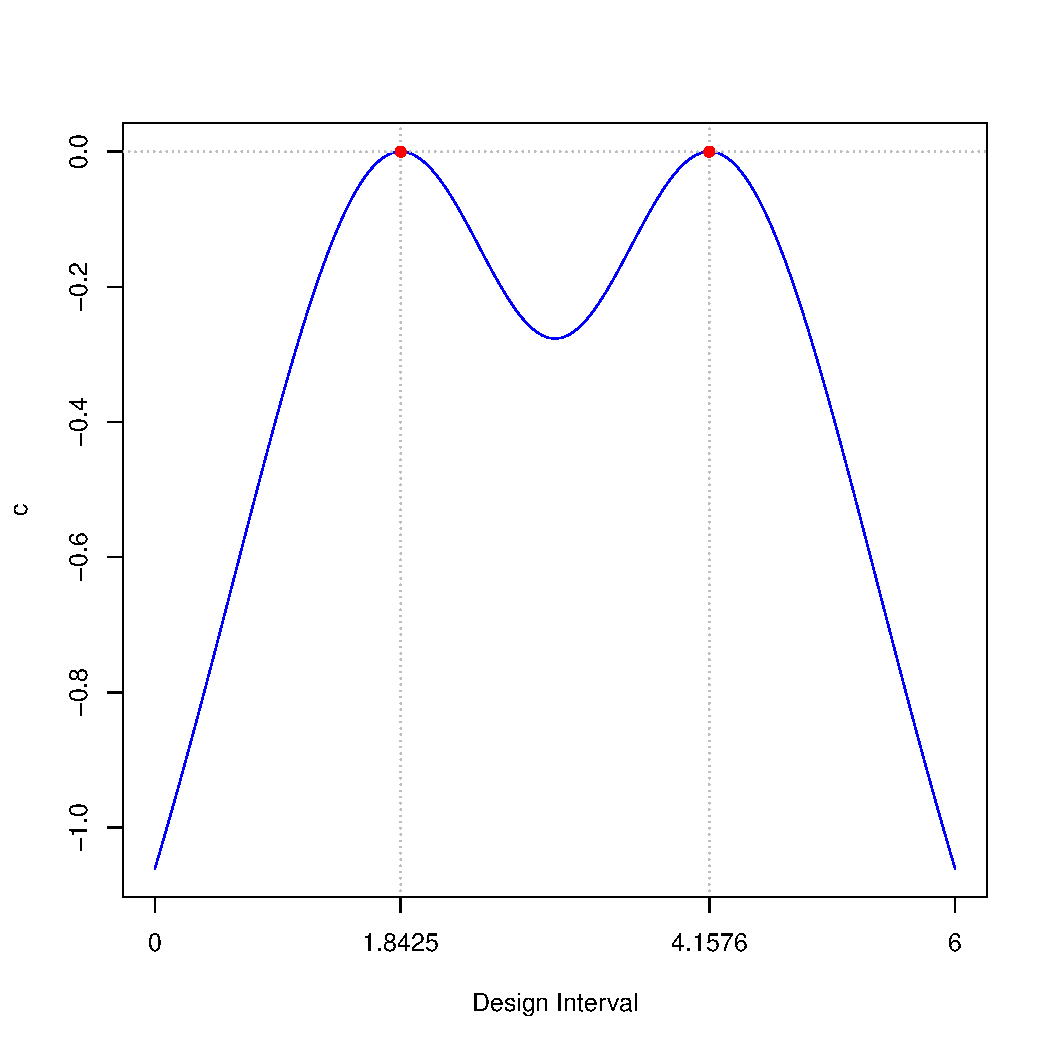
\includegraphics[width=.43\textwidth]{log1.pdf}
}
\subfloat[][\code{Output from plot(log3)}]{
  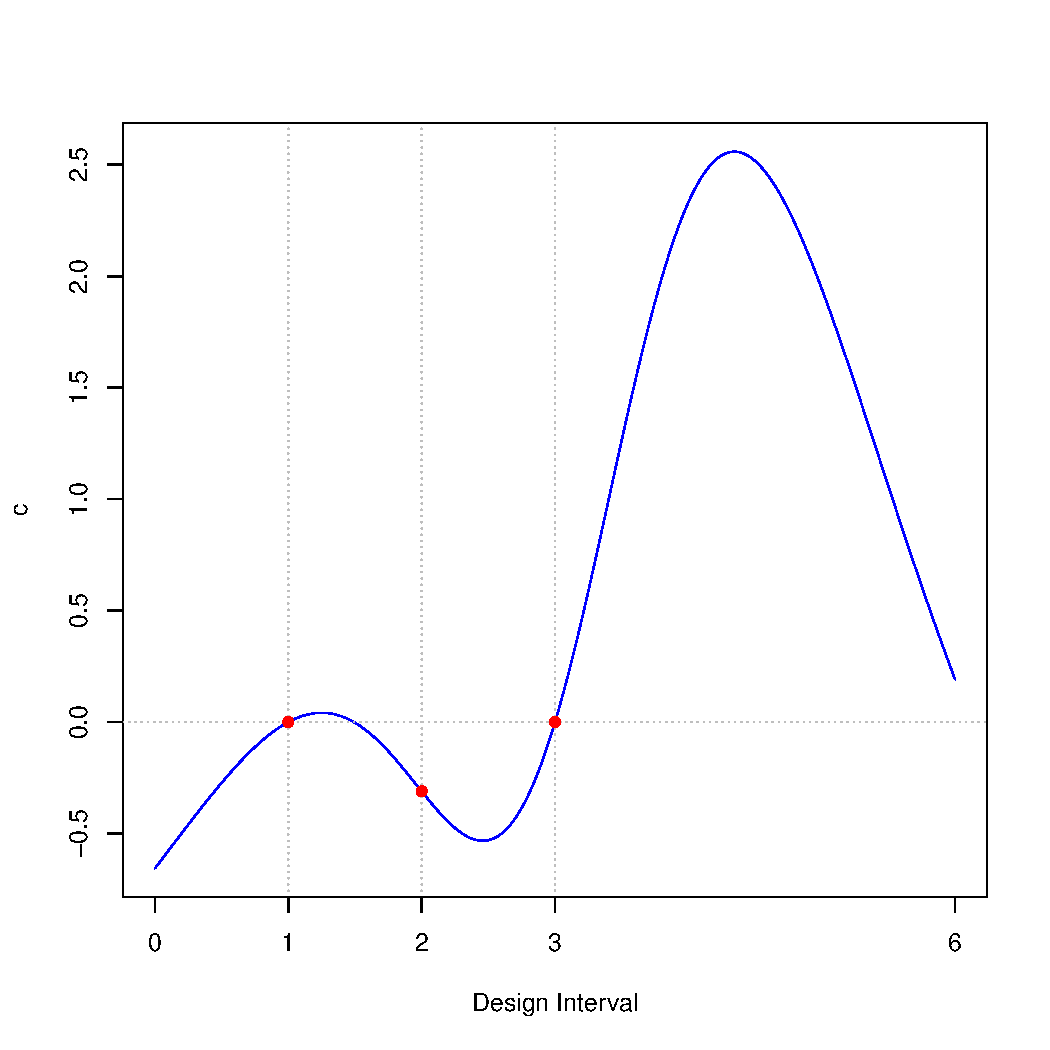
\includegraphics[width=.43\textwidth]{log3.pdf}
}
\caption{
  Plots of the  sensitivity functions  of the designs generated by  the \fct{locally} function for the logistic model over  $\chi =  [0, 6]$ when $\btheta = \btheta_0 =(-4, 1.3333)^T$. The left panel (a) verrfies the global optimality of the obtained design and the right panel (b) does not verify the optimality of the obtained design. The solid red dots are the values of the sensitivity function at the obtained design points.
}
\label{fig:sensitivity-logistic-locally}
\end{figure*}
%%%%%%%%%%%%%%%%%%%%%%%%%%%%%%%%%%%%%


Figure~\ref{fig:sensitivity-logistic-locally} (a) displays the plot of the sensitivity function~\eqref{eq:sensitivity-locally}  of  the design provided by the output on the design space $[0,6]$. Based on the equivalence theorem, this design is optimal because  the sensitivity function is equal or less than zero on $[0,6]$ and (roughly) equal to zero at  $1.84249$ and $4.15765$  (see the red points).  The value of the ELB is nearly $1$, which also indicates the optimality of this design.

It is  interesting to assess the performance of  the uniform design $\xi_{uni}$ with respect to the locally $D-$optimal design obtained above. Using~\eqref{eq:locally-D-efficiency},  we can calculate the $D-$efficiency of  $\xi_{uni}$ relative to the  locally $D-$optimal design by
\begin{example}
R> leff(formula = ~exp(b0 + b1 * x)/(1 + exp(b0 + b1 * x)),
+      predvars = "x", parvars = c("b0", "b1"),
+      family = "binomial", inipars = c(-4, 1.3333),
+      x1 = c(0:6), w1 = rep(1/7, 7),
+      x2 = log1$evol[[20]]$x, w2 = log1$evol[[20]]$w)
[1] 0.7778719
\end{example}
The value of the relative $D-$efficiency indicates  that $\xi_{uni}$ requires about $100(1/0.777-1)= 29\%$ more number of subjects to have the same $D-$efficiency  as the $D-$optimal design when $\btheta = \btheta_0$.  Therefore, having subjects to practice, say, less than 1 hours or more than 5 hours will not increase the efficiency of the parameter estimates very much. 

The value of the ELB  may  also be used to construct a stopping rule condition  for  ICA. This  feature  is activated via the  \code{ICA.control} argument in all OD functions similar to what  follows.
\begin{example}
R> log2 <- locally(formula = ~exp(b0 + b1 * x)/(1 + exp(b0 + b1 * x)),
+                 predvars = "x", parvars = c("b0", "b1"),
+                 family = "binomial", lx = 0, ux = 6, iter = 40, k = 2,
+                 inipars = c(-4, 1.3333),
+                 ICA.control = list(rseed = 1,
+                                    checkfreq = 20,
+                                    stop_rule = "equivalence",
+                                    stoptol = .99))
R> print(log2)
Finding  locally optimal designs

Call:
  ~exp(b0 + b1 * x)/(1 + exp(b0 + b1 * x))

iter       x1       x2        w1        w2 min_cost mean_cost
1     1 1.897630 4.289279 0.4480275 0.5519725 3.585707  3.629564
3     3 1.895518 4.285989 0.4875810 0.5124190 3.575159  3.616086
5     5 1.735791 4.135709 0.4818501 0.5181499 3.574277  3.608956
7     7 1.818028 4.160041 0.4797011 0.5202989 3.570617  3.570617
9     9 1.812077 4.132323 0.4965689 0.5034311 3.569134  3.569134
11   11 1.827779 4.137145 0.4958561 0.5041439 3.568919  3.568919
13   13 1.844558 4.142393 0.4961667 0.5038333 3.568856  3.568856
15   15 1.845992 4.165776 0.4984264 0.5015736 3.568713  3.568713
17   17 1.845348 4.155565 0.4996783 0.5003217 3.568688  3.568688
20   20 1.842781 4.159234 0.4999992 0.5000008 3.568680  3.568680

Optimal designs (k=2):
  Points1 Points2
1.84278 4.15923
Weights1 Weights2
0.500   0.500

ICA iteration: 20
Criterion value:  3.56868
Total number of function evaluations: 918
Total number of successful local search moves: 46
Total number of successful revolution moves: 46
Convergence: equivalence
Total number of successful assimilation moves: 345
CPU time: 0.81  seconds!
  
  Maximum of the sensitivity function is  3.483904e-06
Efficiency lower bound (ELB) is  0.9999983
Verification required 0.39 seconds!
  R> log2$design
iter       x1       x2        w1        w2 min_cost mean_cost     max_sens
1   20 1.842781 4.159234 0.4999992 0.5000008  3.56868   3.56868 3.483904e-06
elb time_sec
1 0.9999983     0.39
\end{example}

We set \texttt{stop\_rule} = \code{"equivalence"} to activate the stopping rule that is based on the equivalence theorem. In this case,  ICA starts to  calculate the ELB for the best design every \code{checkfreq} = 20 iterations  and it  stops whenever the value of the ELB is larger than  \code{stoptol} = 0.99.  In this example, ICA stopped at the first check run because the value of ELB is 0.999 (> \code{stoptol}).
%%$0.999 (> \mbox{\texttt{stoptol}})$.
Note that we requested to calculate the ELB after every 20 iterations, instead of every iteration, to prevent a significant increase in the CPU time.
This equivalence-based  stopping rule is  also available in other OD functions. However, we note that optimality verification  for  Bayesian or   minimax   type criteria is more complicated and may slow down the ICA.


\CRANpkg{ICAOD} can also handle a situation where the design points are pre-specified, but their optimal associated weights are of interest.
For example,  assume that the experimental  resources only allow a pre-specified hours of practice, say,   $x_1 = 1$, $x_2 = 2$, $x_3 = 3$ hours. In all OD functions, the design points can be specified  similarly via the argument \code{x} (a vector of design points):
  \begin{example}
R> log3 <- locally(formula = ~exp(b0 + b1 * x)/(1 + exp(b0 + b1 * x)),
+                 predvars = "x", parvars = c("b0", "b1"),
+                 family = "binomial", lx = 0, ux = 6, iter = 40,
+                 x = c(1, 2, 3),
+                 inipars = c(-4, 1.3333),
+                 ICA.control = list(rseed = 1, checkfreq = Inf))

R> print(log3)
Finding  locally optimal designs

Call:
  ~exp(b0 + b1 * x)/(1 + exp(b0 + b1 * x))

iter x1 x2 x3        w1           w2        w3 min_cost mean_cost
1     1  1  2  3 0.4528099 2.460808e-03 0.5447293 4.196368  4.205840
5     5  1  2  3 0.5106454 5.660663e-03 0.4836939 4.190011  4.190011
9     9  1  2  3 0.4993132 8.104013e-05 0.5006058 4.187368  4.187368
14   14  1  2  3 0.4993694 9.602963e-06 0.5006210 4.187346  4.187346
18   18  1  2  3 0.4998314 4.227502e-06 0.5001644 4.187343  4.187343
22   22  1  2  3 0.4998286 1.079043e-07 0.5001713 4.187342  4.187342
27   27  1  2  3 0.4999951 1.656952e-08 0.5000049 4.187342  4.187342
31   31  1  2  3 0.4999982 4.628899e-10 0.5000018 4.187342  4.187342
35   35  1  2  3 0.4999994 5.689118e-11 0.5000006 4.187342  4.187342
40   40  1  2  3 0.5000001 2.449702e-12 0.4999999 4.187342  4.187342

Optimal designs (k=3):
  Weights: 0.500 0.000 0.500

ICA iteration: 40
Criterion value:  4.187342
Total number of function evaluations: 1731
Total number of successful local search moves: 39
Total number of successful revolution moves: 30
Convergence: Maximum_Iteration
Total number of successful assimilation moves: 878
CPU time: 1.22  seconds!
  
  Maximum of the sensitivity function is  2.558775
Efficiency lower bound (ELB) is  0.4387143
Verification required 0.35 seconds!
  \end{example}
The results show that  no weight should be assigned to the subjects with 2 hours of practice. This means that, the responses from subjects with 2 hours of practice  will not increase  the efficiency of estimation very much. Hence, this level may be eliminated  to save more resources.

The value of the ELB and the plot of the sensitivity function in Figure~\ref{fig:sensitivity-logistic-locally} (b) clearly  show that the obtained design is not  globally optimal. This comes as no surprise because the given design points in \code{x} do not belong to the  support of the optimal design when $\btheta = \btheta_0$.
Note that \code{checkfreq = Inf} requests a \code{plot} method for the design provided by the output  so that \fct{plot} is not required anymore. For space consideration, we use this option in the rest of this paper.


Locally optimal designs usually lose their efficiency  when the parameter estimates are far from their true unknown values.
Moreover, in practice, it is more realistic to assume that the parameters belong to a  parameter space, rather than fixing their values at some points. For example, let    $\btheta = (\beta_0, \beta_1)^T$ belongs to $\Theta = [\beta_0^L, \beta_0^U] \times [\beta_1^L, \beta_1^U]$, where $\beta_0^L = -6$,  $\beta_0^U = -2$, $\beta_1^L = .5$ and $\beta_1^U = 2$.
As  a conservative strategy, a  minimax $D-$optimal design   minimizes the maximum inefficiency over $\Theta$.
To find the minimax $D-$optimal design for our design setting, we first set $k = 2$ to find  the minimax $D-$optimal design within the class of two-point designs:
  \begin{example}
R> log4 <- minimax(formula = ~exp(b0 + b1 * x)/(1 + exp(b0 + b1 * x)),
+                 predvars = "x", parvars = c("b0", "b1"),
+                 family = "binomial",
+                 lx = 0, ux = 6, lp = c(-6, .5), up = c(-2, 2),
+                 iter = 200, k = 2,
+                 ICA.control = list(rseed = 1,
+                                    checkfreq = 50,
+                                    stop_rule = "equivalence",
+                                    stoptol = .99),
+                 crt.minimax.control = list(optslist = list(maxeval = 200)))
R> print(log4)
Finding  minimax optimal designs

Call:
  ~exp(b0 + b1 * x)/(1 + exp(b0 + b1 * x))

iter        x1       x2        w1        w2 min_cost mean_cost
1      1 0.4446832 4.868664 0.4243584 0.5756416 7.853582  8.061686
23    23 0.7665387 4.895727 0.4965758 0.5034242 7.782827  7.782827
45    45 0.7639494 4.895787 0.4999084 0.5000916 7.782754  7.782754
67    67 0.7636147 4.895791 0.5000079 0.4999921 7.782754  7.782754
89    89 0.7636144 4.895791 0.5000079 0.4999921 7.782754  7.782754
111  111 0.7636144 4.895791 0.5000079 0.4999921 7.782754  7.782754
133  133 0.7635408 4.895792 0.4999934 0.5000066 7.782754  7.782754
155  155 0.7635408 4.895792 0.4999934 0.5000066 7.782754  7.782754
177  177 0.7635408 4.895792 0.4999934 0.5000066 7.782754  7.782754
200  200 0.7635408 4.895792 0.4999934 0.5000066 7.782754  7.782754

Optimal designs (k=2):
  Points1 Points2
0.76354 4.89579
Weights1 Weights2
0.500   0.500

ICA iteration: 200
Criterion value:  7.782754
Total number of function evaluations: 1710132
Total number of successful local search moves: 120
Total number of successful revolution moves: 60
Convergence: Maximum_Iteration
Total number of successful assimilation moves: 1007
Vector of maximum parameter values:  -6 0.5
CPU time: 211.47  seconds!
  
  Maximum of the sensitivity function is  21.9395
Efficiency lower bound (ELB) is  0.08354392
Verification required 0.72 seconds!
  Adjust the control parameters in 'sens.minimax.control' ('n_seg')
or in 'sens.bayes.control' for higher speed.
\end{example}
To increase the CPU time, we reduced the value of \code{maxeval} from $1000$ (default value) to $200$.
Figure~\ref{fig:sensitivity-logistic-minimax} (a) displays the sensitivity plot of the design by provided by the output and it does not verify  the optimality of the two-point design.
%%%%%%%%%%%%%%%%%%%%%%%%%%%%%%%%%%%%%%%%%%%%%%%%%%%
\begin{figure*}[t!]
\centering
\subfloat[][$k = 2$]{
  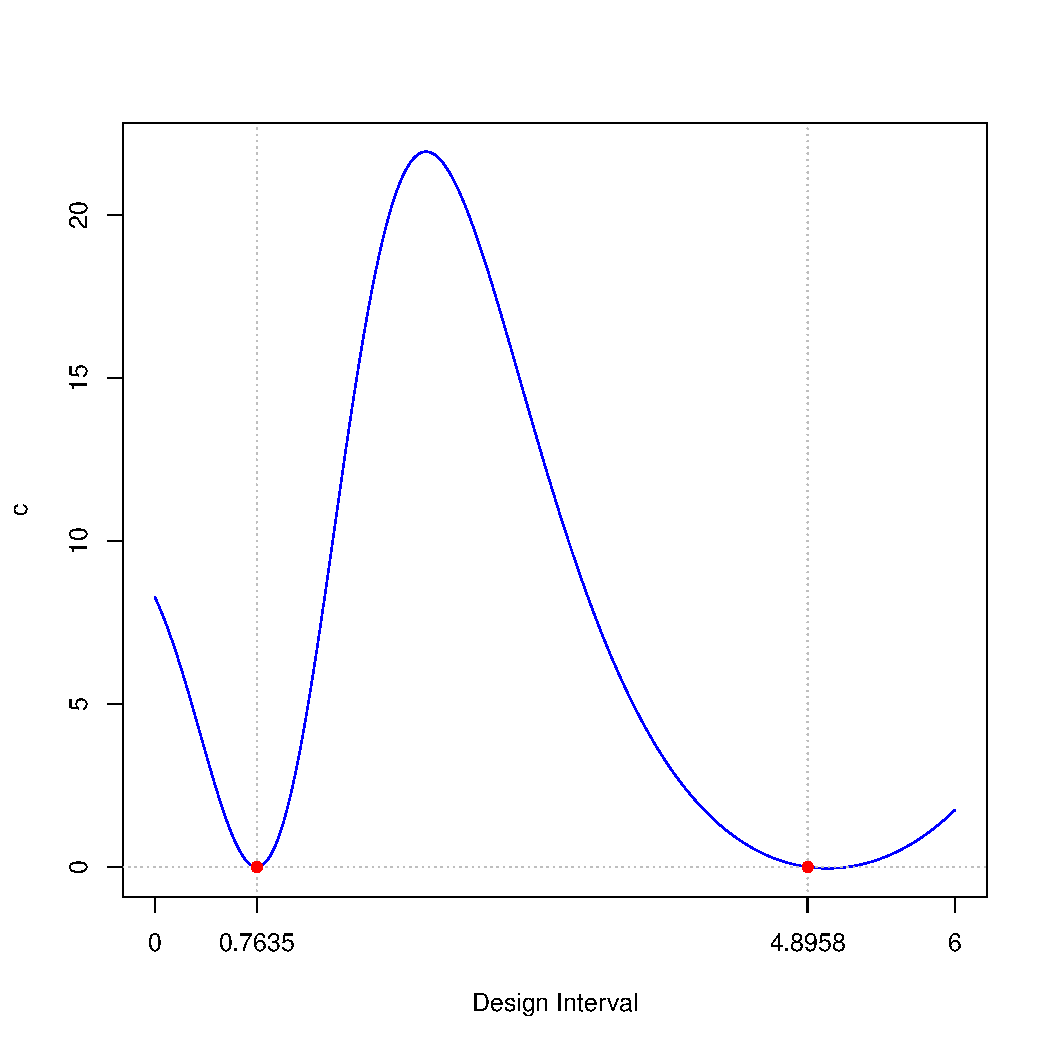
\includegraphics[width=.43\textwidth]{log4.pdf}
}
\subfloat[][$k = 3$]{
  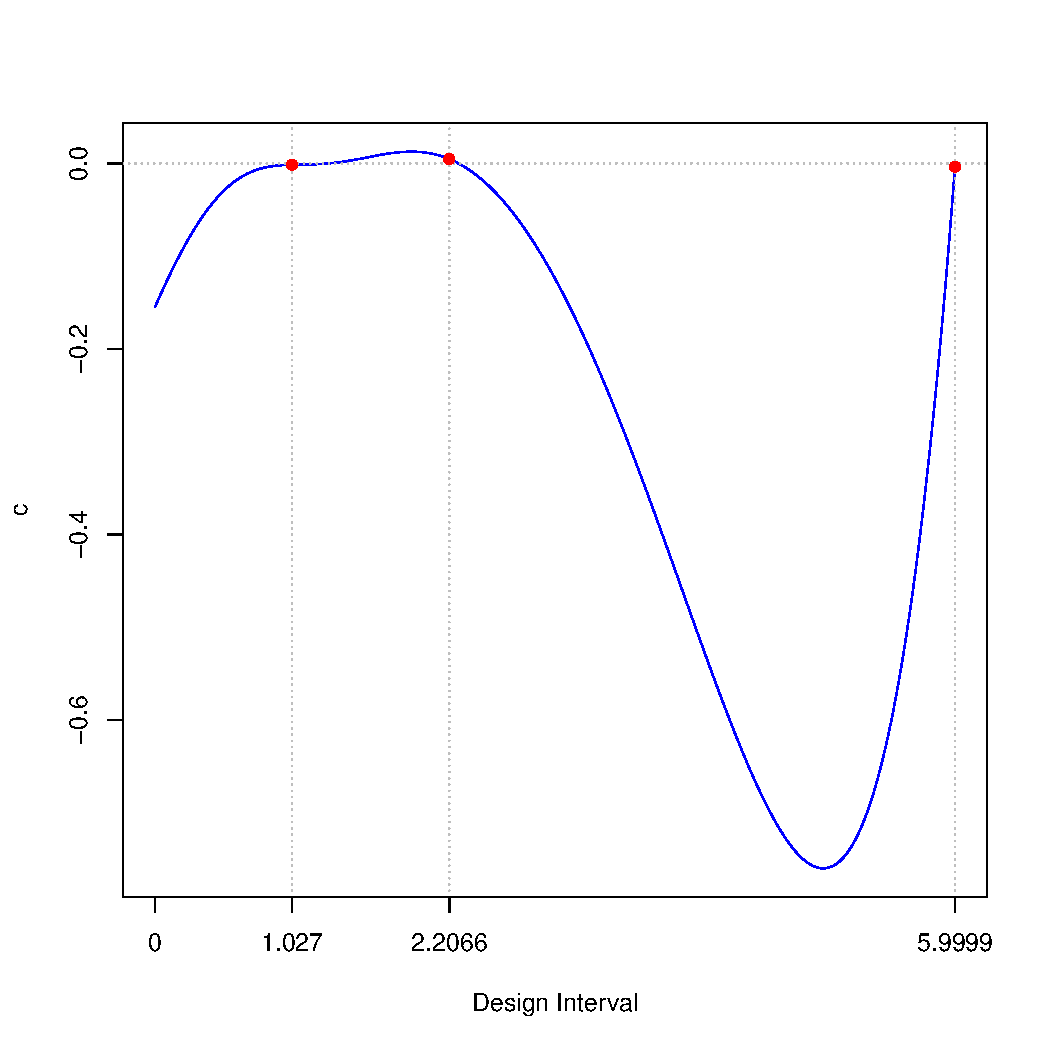
\includegraphics[width=.43\textwidth]{log5.pdf}
}\\
\caption{
  Plots of the  sensitivity functions of  the two- and three-point designs generated by the  \fct{minimax} function for the logistic regression model over $ \chi = [0, 6]$ when $\Theta = [-6, -2]\times[0.5, 2]$.  The left panel (a) does not verifies the optimality of the obtained design and the right panel (b) shows the nearly optimality of the three-point design.  The solid red dots are the values of the sensitivity function at the obtained design points.
}
\label{fig:sensitivity-logistic-minimax}
\end{figure*}
%%%%%%%%%%%%%%%%%%%%%%%%%%%%%%%%%%%%%%%%%%%%%%%%%%%
Therefore, we increment the value of $k$ by one and re-execute the above code:
  \begin{example}
R> log5 <- minimax(formula = ~exp(b0 + b1 * x)/(1 + exp(b0 + b1 * x)),
+                 predvars = "x", parvars = c("b0", "b1"),
+                 family = "binomial",
+                 lx = 0, ux = 6, lp = c(-6, .5), up = c(-2, 2),
+                 iter = 500, k = 3,
+                 ICA.control = list(rseed = 1,
+                                    checkfreq = 50,
+                                    stop_rule = "equivalence",
+                                    stoptol = .99),
+                 crt.minimax.control = list(optslist = list(maxeval = 200)))
R> print(log5)
Finding  minimax optimal designs

Call:
  ~exp(b0 + b1 * x)/(1 + exp(b0 + b1 * x))

iter        x1       x2       x3        w1        w2        w3 min_cost
1     1 1.0613974 2.577126 5.994463 0.1263308 0.5337391 0.3399301 6.862938
6     6 0.9212932 2.161076 5.999569 0.1092450 0.5392481 0.3515069 6.826309
11   11 0.9291691 2.163344 5.998872 0.1131382 0.4602769 0.4265849 6.760707
17   17 0.9358663 2.165053 5.998143 0.1131382 0.4602769 0.4265849 6.758872
22   22 1.0343686 2.163586 5.997440 0.1000379 0.4592324 0.4407297 6.749718
28   28 1.1201234 2.340084 5.995084 0.1526103 0.3628279 0.4845619 6.745782
33   33 1.0084352 2.232590 5.999449 0.1185027 0.3770129 0.5044843 6.738361
39   39 1.0003813 2.245542 5.999894 0.1094120 0.3941922 0.4963958 6.737553
44   44 1.0159978 2.225392 5.999982 0.1148592 0.3916467 0.4934942 6.737084
50   50 1.0269974 2.206648 5.999927 0.1135038 0.3915064 0.4949898 6.736338
mean_cost
1   7.553929
6   6.951918
11  6.805511
17  6.776728
22  6.757709
28  6.748353
33  6.743650
39  6.742541
44  6.738447
50  6.737655

Optimal designs (k=3):
  Points1 Points2 Points3
1.02700 2.20665 5.99993
Weights1 Weights2 Weights3
0.114   0.392   0.495

ICA iteration: 50
Criterion value:  6.736338
Total number of function evaluations: 511836
Total number of successful local search moves: 309
Total number of successful revolution moves: 92
Convergence: equivalence
Total number of successful assimilation moves: 407
Vector of maximum parameter values:  -6 0.5
CPU time: 71.04  seconds!
  
  Maximum of the sensitivity function is  0.01269528
Efficiency lower bound (ELB) is  0.9936924
Verification required 2.16 seconds!
  Adjust the control parameters in 'sens.minimax.control' ('n_seg')
or in 'sens.bayes.control' for higher speed.
R> log5$design
iter       x1       x2       x3        w1        w2        w3 min_cost
1   50 1.026997 2.206648 5.999927 0.1135038 0.3915064 0.4949898 6.736338
mean_cost   max_sens       elb time_sec
1  6.737655 0.01269528 0.9936924     2.16
\end{example}


Figure~\ref{fig:sensitivity-logistic-minimax} (b) displays the plot of the sensitivity function of the three-point generated design and it  indicates its nearly optimality.  
The optimal design  suggests subjects with nearly $1$, $2$ and $6$ hours of practice, where roughly half of the subjects should be  assigned to practice for $6$ hours.


Similar to the locally $D-$optimal design, we can assess the minimax $D-$efficiency of $\xi_{uni}$ with respect to the minimax $D-$optimal design by
\begin{example}
R> meff(formula = ~exp(b0 + b1 * x)/(1 + exp(b0 + b1 * x)),
+      predvars = "x", parvars = c("b0", "b1"),
+      family = "binomial",
+      lp = c(-6, .5), up = c(-2, 2),
+      x1 = c(0:6), w1 = rep(1/7, 7),
+      x2 = log5$evol[[20]]$x, w2 = log5$evol[[20]]$w)
[1] 0.7459795
\end{example}
This value indicates that  $\xi_{uni}$ requires about $100(1/0.74089-1) = 35\%$ more subjects to have the same minimax $D-$efficiency  as the minimax $D-$optimal design  when $\Theta = [-6, -2]\times[0.5, 2]$.


\subsection{Sigmoid-Emax model}
\label{sec:sigmoid}
The sigmoid Emax model is commonly used in pharmacokinetics/pharamacodynamics to describe the S-shape dose-response relationship \citep[see, e.g.,][]{ Macdougall2006, Thomas2006}.
This model  is defined by
\begin{equation}
\label{eq:sigmoid-Emax}
E(Y) = f(x, \btheta) = \beta_1 + (\beta_2-\beta_1) \frac{x^{\beta_4}}{x^{\beta_4} + \beta_3^{\beta_4}},
\end{equation}
where $x$ is the dose level (in mg), $x \in \chi = (0, x_0]$, $x_0$ is user-selected and  $\btheta = (\beta_1, \beta_2, \beta_3, \beta_4)^T$, $\theta_2>\beta_1$,  $\beta_3>0$.
All  errors  are assumed to be independent and normally distributed with mean zero and constant variance. Here, $\beta_1$ is the minimum mean response, $\beta_2$ is the maximum mean response, $\beta_3$ is the ED50, i.e., the dose at which $50$ percent of the maximum mean effect is achieved, and $\beta_4$ is the slope parameter.



In dose-response studies, optimal designs  usually  determine how many doses are required to be tested, what are their levels, and how many subjects to allocate to each dose level.
Let  $\chi = (0, 1000]$mg.
Similar to \citet{dragalin2007adaptive} and \citet{wang2014adaptive}, we are interested in the efficient estimation of $\btheta$ and the $D-$optimality  is an appropriate design criterion for this purpose.

It  is straightforward to show that the  FIM of the sigmoid Emax model depends on the unknown parameters $\btheta$. This parameter dependency must be dealt with based on the  type of information available on $\btheta$.
For example, using information from a  pilot study,  one may elicit a uniform prior distribution  for $\btheta$ and search for Bayesian optimal designs.
As an illustrative example, let $\beta_1 \sim U(4, 8)$, $\beta_2 \sim U(11, 15)$, $\beta_3 \sim U(100, 130)$ and $\beta_4 \sim U(5, 9)$,  and all the uniform prior distributions be independent.
For simplicity,  we denote the independent uniform distributions for $\beta_i, i = 1, 2,3, 4$ by $\pi_{\Theta}$,   where $\Theta = [4, 8] \times [11, 15] \times[100,130] \times [5, 9] $ is the parameter space. This prior can be defined in \CRANpkg{ICAOD} by the \fct{uniform}  function as follows.
\begin{example}
R> prior1 <- uniform(lower = c(4, 11, 100, 5), upper = c(8, 15, 130, 9))
\end{example}
Here, the output is an object  of class \class{cprior}, which can be passed to the argument \code{prior} of  the \fct{bayes} function.


To find the number of support points for the Bayesian $D-$optimal design, we repeated the same incremental process %as described in the section \samp{Logistic Model with A Single Predictor} %Section~\ref{sec:logsitc-single} 
for finding minimax optimal design. This process is  excluded here due to space consideration.  The Bayesian $D-$optimal design has $5$ points in its support, which are found by
\begin{example}
R> sig1 <- bayes(formula = ~b1 + (b2-b1) * x^b4/(x^b4 + b3^b4),
+               predvars = "x",
+               parvars = c("b1", "b2", "b3", "b4"),
+               lx = .001, ux = 1000, k = 5, iter = 400, prior = prior1,
+               ICA.control = list(rseed = 1, checkfreq = Inf))
R> print(sig1)
Finding  Bayesian optimal designs

Call:
  ~b1 + (b2 - b1) * x^b4/(x^b4 + b3^b4)

iter         x1       x2       x3       x4        x5        w1        w2
1      1 18.0475346 96.25014 167.5667 179.3485  867.8058 0.2909521 0.1581145
45    45 17.4961312 89.11527 108.3659 137.0731  866.5956 0.2368958 0.1548766
89    89  0.4786294 95.25557 115.0471 138.2732  554.3556 0.2460043 0.2036432
134  134  1.0415205 94.75054 113.8961 138.3159  959.5441 0.2430275 0.1959315
178  178  0.7994201 94.64836 113.7667 138.3264  999.8505 0.2433772 0.1949845
222  222  1.8666601 94.60760 113.7090 138.3516  999.9069 0.2432310 0.1942385
267  267  0.5492615 94.60194 113.7011 138.3539  999.9987 0.2432085 0.1941306
311  311  0.4263460 94.60176 113.6966 138.3513 1000.0000 0.2432061 0.1941301
355  355  0.4164132 94.60189 113.6965 138.3510 1000.0000 0.2432041 0.1941322
400  400  0.1805450 94.60188 113.6964 138.3510 1000.0000 0.2432040 0.1941319
w3          w4        w5 min_cost mean_cost
1   0.3418695 0.006883086 0.2021808 14.10396  15.82570
45  0.1428410 0.225597557 0.2397890 12.74113  12.74774
89  0.1043130 0.200569541 0.2454699 12.72302  12.72989
134 0.1140765 0.203490785 0.2434737 12.72086  12.72095
178 0.1150226 0.203128842 0.2434868 12.72082  12.72083
222 0.1158376 0.203138347 0.2435545 12.72082  12.72082
267 0.1159406 0.203152463 0.2435679 12.72082  12.72082
311 0.1159200 0.203173666 0.2435701 12.72082  12.72082
355 0.1159159 0.203177516 0.2435702 12.72082  12.72082
400 0.1159155 0.203178189 0.2435705 12.72082  12.72082

Optimal designs (k=5):
  Points1    Points2    Points3    Points4    Points5
0.18055    94.60188   113.69639  138.35096  1000.00000
Weights1   Weights2   Weights3   Weights4   Weights5
0.243      0.194      0.116      0.203      0.244

ICA iteration: 400
Criterion value:  12.72082
Total number of function evaluations: 85150
Total number of successful local search moves: 2378
Total number of successful revolution moves: 81
Convergence: maxiter
Total number of successful assimilation moves: 1700
CPU time: 611.44  seconds!
  
  Maximum of the sensitivity function is  9.439815e-07
Efficiency lower bound (ELB) is  0.9999998
Verification required 65.3 seconds!
  Adjust the control parameters in 'sens.minimax.control' ('n_seg')
or in 'sens.bayes.control' for higher speed.
R> sig1$design
iter       x1       x2       x3      x4   x5       w1        w2        w3
1  400 0.180545 94.60188 113.6964 138.351 1000 0.243204 0.1941319 0.1159155
w4        w5 min_cost mean_cost     max_sens       elb time_sec
1 0.2031782 0.2435705 12.72082  12.72082 9.439815e-07 0.9999998     65.3
\end{example}

%%%%%%% %%%%%%%%


Figure~\ref{fig:sensitivity-sigmoid-bayes} (a) is generated from the output and presents the plot of the  sensitivity function of the five-point design and it verifies its  optimality.
In our example, the Bayesian $D-$optimal design suggests five dose levels, with four of them located below $140$mg and one located at the maximum. Roughly $50\%$ of the observations should be assigned to the lower and upper bound of the dose interval.
Note that the result can also be obtained in  lesser CPU time if we  adjust the control  parameters of the integral approximations via the argument \code{crt.bayes.control}.
%For a discussion on these tuning parameters,  see \citet{masoudi2019}.

Using a non-optimal design may  be  inefficient even when its  design points are sampled uniformly from the design space. As an illustrative example, assume a situation where  a researcher decides  to work with an equally-weighted uniform design that has $11$ points located on $0.001, 100, 200, 300, ....,1000$. This design is not  optimal when $\btheta \sim \pi_\Theta$.
The  Bayesian $D-$efficiency  of the uniform design with respect to the obtained Bayesian $D-$optimal design is calculated by
\begin{example}
R> beff(formula = ~b1 + (b2-b1) * x ^b4/(x^b4 + b3^b4),
+      predvars = "x",
+      parvars = c("b1", "b2", "b3", "b4"),
+      prior = prior1,
+      x1 = c(.001,seq(100, 1000, by = 100)),
+      w1 = rep(1/11, 11),
+      x2 = sig1$evol[[400]]$x, w2 = sig1$evol[[400]]$w)
[1] 0.3063289
\end{example}

The non-optimal design may seem reasonable,  but its Bayesian $D-$efficiency value suggests that, roughly $226\%$ more observations are needed to maintain the $D-$efficiency for the non-optimal design in comparison to the Bayesian $D-$optimal design when
$\btheta \sim \pi_\Theta$. The \fct{bayes} function  is very  flexible and  can incorporate different   prior distributions. %For more details, see \citet{masoudi2019}.

\CRANpkg{ICAOD} can also  find robust or optimum-on-average designs when the prior distributions  are  discrete. As an illustrative example,  assume $\Theta_0 = \{\btheta_{01}, \btheta_{02} , \btheta_{03} , \btheta_{04} , \btheta_{05}\}$ be a set of five vectors of  initial estimates  for $\btheta = (\beta_1, \beta_2,\beta_3, \beta_4)$, where  $\btheta_{01} = (4, 11, 100, 5)$, $ \btheta_{02} = (5, 12, 110, 6)$, $\btheta_{03} = (6, 13, 120, 7)$, $\btheta_{04} = (8, 15, 130, 9)$ and $\btheta_{05} = (12, 30, 160, 13)$. Let $\pi_{\Theta_0}$ denotes a discrete uniform  prior distribution that assigns the same probability to each vector element of  $\Theta_0$. The six-point optimum-on-average design is given by
\begin{example}
R> parset1 <- matrix(c(4, 11, 100, 5,
+                     5, 12, 110, 6,
+                     6, 13, 120, 7,
+                     8, 15, 130, 9,
+                     12, 30, 160, 13),
+                   nrow = 5, byrow = TRUE)
R> sig2 <- robust(formula = ~b1 + (b2-b1) * x ^b4/(x^b4 + b3^b4),
+                predvars = "x",
+                parvars = c("b1", "b2", "b3", "b4"),
+                lx = .001, ux = 1000, k = 6, iter = 400,
+                parset = parset1,
+                prob = rep(1/5, 5),
+                ICA.control = list(rseed = 1, checkfreq = Inf))
R> print(sig2)
Finding  robust or optimum-on-average optimal designs

Call:
  ~b1 + (b2 - b1) * x^b4/(x^b4 + b3^b4)

iter          x1       x2       x3       x4       x5        x6        w1
1      1 52.47474098 86.13143 108.6089 176.5576 847.1196  865.1056 0.3356308
45    45  0.03699118 93.84970 115.0752 144.3279 172.2496  612.5133 0.1921861
89    89  0.26057011 86.13743 112.6560 143.7663 170.6661  899.7495 0.1938690
134  134  0.27440675 86.41506 112.7178 143.7321 170.5697  999.4115 0.1997277
178  178  0.42978429 86.41957 112.7179 143.7262 170.5713  999.5817 0.2001652
222  222  0.86217693 86.41953 112.7092 143.7262 170.5733  999.9999 0.2001538
267  267  0.78134061 86.42156 112.7098 143.7250 170.5722 1000.0000 0.2001708
311  311  0.28372653 86.42155 112.7098 143.7248 170.5723 1000.0000 0.2001738
355  355  0.08123600 86.42156 112.7099 143.7248 170.5723 1000.0000 0.2001734
400  400  0.04980091 86.42158 112.7099 143.7248 170.5723 1000.0000 0.2001734
w2        w3        w4         w5        w6 min_cost mean_cost
1   0.06870259 0.1056298 0.2022530 0.12858302 0.1592008 14.10402  16.35115
45  0.15186984 0.1444531 0.2155502 0.08196997 0.2139708 12.25422  12.31711
89  0.13222946 0.1570768 0.1882862 0.09776625 0.2307723 12.21447  12.28391
134 0.13190606 0.1549309 0.1855214 0.09816873 0.2297452 12.21398  12.28328
178 0.13154222 0.1547794 0.1858112 0.09840028 0.2293017 12.21398  12.28311
222 0.13149988 0.1548130 0.1857954 0.09845378 0.2292841 12.21398  12.28305
267 0.13150916 0.1547914 0.1857821 0.09847028 0.2292762 12.21398  12.27535
311 0.13150554 0.1547882 0.1857820 0.09847434 0.2292761 12.21398  12.26001
355 0.13150671 0.1547883 0.1857817 0.09847396 0.2292760 12.21398  12.21398
400 0.13150681 0.1547882 0.1857817 0.09847394 0.2292759 12.21398  12.21398

Optimal designs (k=6):
  Points1    Points2    Points3    Points4    Points5    Points6
0.04980    86.42158   112.70988  143.72485  170.57227  1000.00000
Weights1   Weights2   Weights3   Weights4   Weights5   Weights6
0.200      0.132      0.155      0.186      0.098      0.229

ICA iteration: 400
Criterion value:  12.21398
Total number of function evaluations: 20070
Total number of successful local search moves: 3787
Total number of successful revolution moves: 88
Convergence: Maximum_Iteration
Total number of successful assimilation moves: 1895
CPU time: 29.56  seconds!
  
  Maximum of the sensitivity function is  3.960066e-07
Efficiency lower bound (ELB) is  0.9999999
Verification required 2.27 seconds!
  R> sig2$design
iter         x1       x2       x3       x4       x5   x6        w1        w2
1  400 0.04980091 86.42158 112.7099 143.7248 170.5723 1000 0.2001734 0.1315068
w3        w4         w5        w6 min_cost mean_cost     max_sens
1 0.1547882 0.1857817 0.09847394 0.2292759 12.21398  12.21398 3.960066e-07
elb time_sec
1 0.9999999     2.27
\end{example}

%%%%%%%%%%%%%%%%%%%%%%%%%%%%%%%%%%%%%%%%%%%%%%%%%%%
\begin{figure*}[h!]
\centering
\subfloat[][$\btheta \sim \pi_{\Theta}$]{
  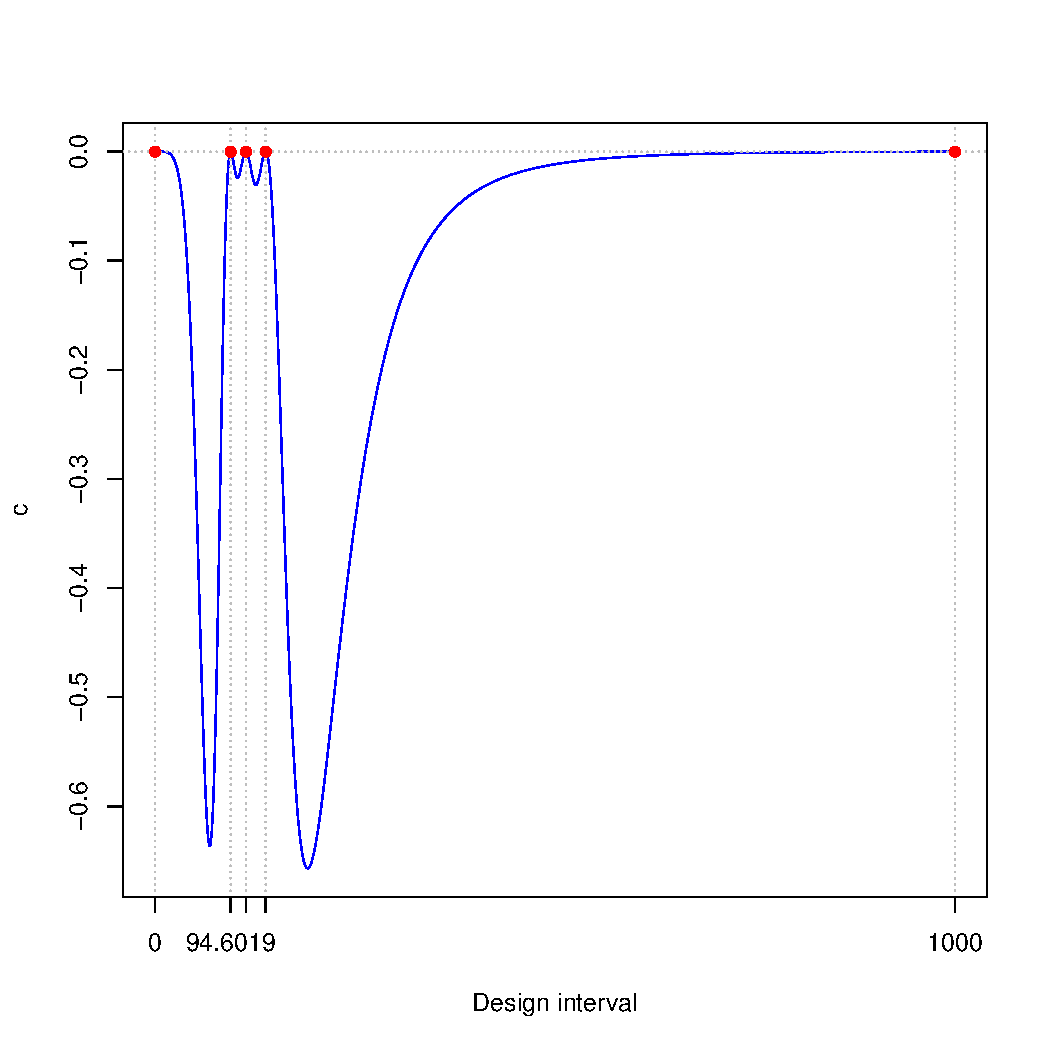
\includegraphics[width=.5\textwidth]{sig1.pdf}
}
\subfloat[][$\btheta \sim \pi_{\Theta_0}$]{
  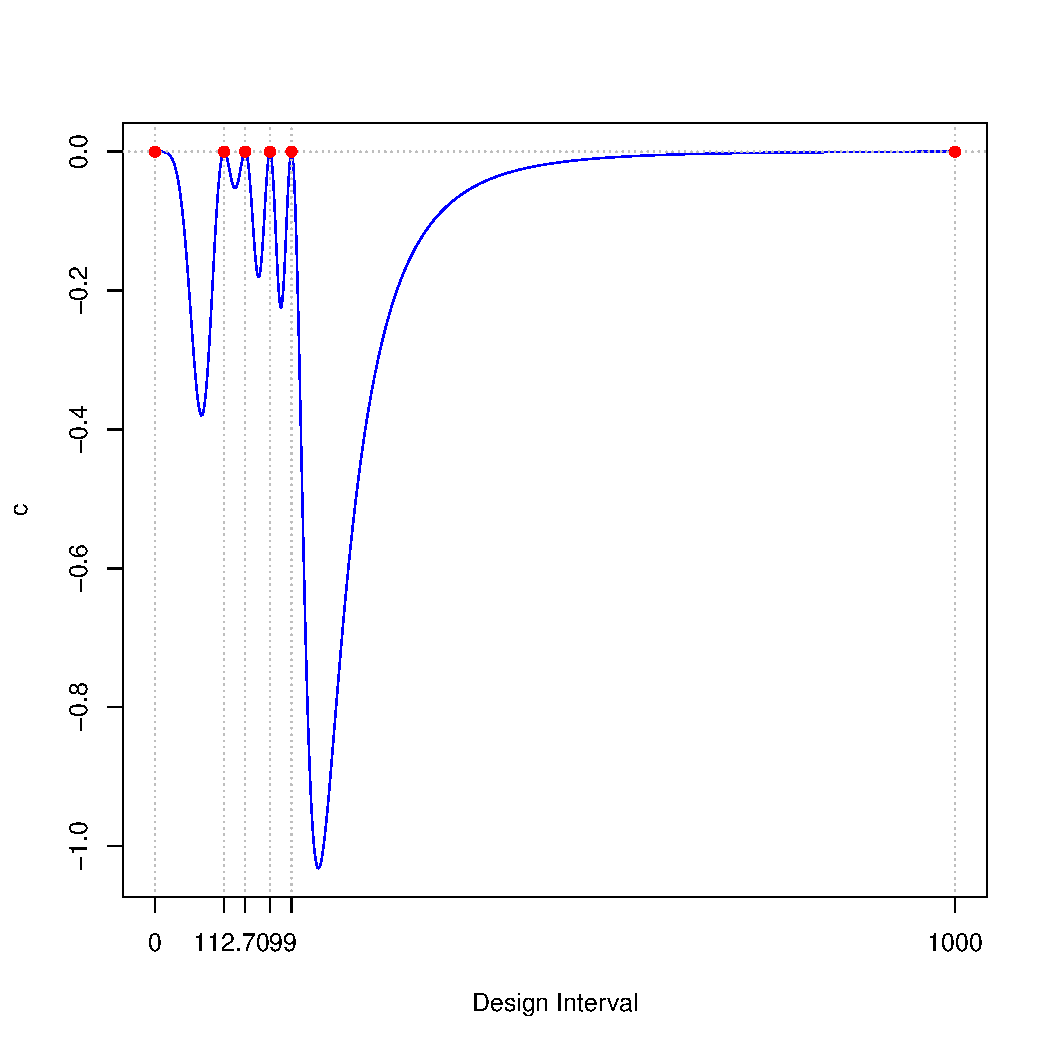
\includegraphics[width=.5\textwidth]{sig2.pdf}
}
\caption{
  The  plots of sensitivity functions  of  the generated designs  for the sigmoid Emax model  over the design space $ [0.001, 1000]$.
  The left panel (a) displays the plot of the sensitivity function of the design generated  by the  function \fct{bayes}   when $\btheta \sim \pi_{\Theta}$. The right panel (b) displays the plot of the sensitivity function of the design generated  by the function \fct{robust}  when $\btheta \sim \pi_{\Theta_0}$. Both (a) and (b) verify the optimality of the obtained design. The solid red dots are the values of the sensitivity function at the obtained design points.  
}
\label{fig:sensitivity-sigmoid-bayes}
\end{figure*}
%%%%%%%%%%%%%%%%%%%%%%%%%%%%%%%%%%%%%%%%%%%%%%%%%%%

Figure~\ref{fig:sensitivity-sigmoid-bayes} (b) displays the  plot of the  sensitivity function of  the design provided by the output  and it verifies the optimality of the six-point design.
Similar to the optimal design generated by \fct{bayes}, the generated design here allocates most of its support points to the lower half of the dose interval.


\section{User-specified optimality criteria}
\label{sec:new-optimality}
\CRANpkg{ICAOD} can also find optimal designs with respect to  user-specified optimality criteria.   In this section, as an illustrative example, we  find $c-$optimal designs for  the two-parameter logistic (2PL) model with applications in dose-response studies.
The 2PL model is commonly used in dose-response studies   to  model the relationship between the dose level of a drug and the probability of  a success, e.g.,  the probability that patients are cured. This model is defined by
\begin{equation}
\label{eq:logistic-model}
f(x, \btheta) = P(Y=1) =  \frac{1}{1 + \exp(-b(x-a))},
\end{equation}
where  $x$ is the dose level (predictor), $\btheta = (a, b)^T$,  $b$ is the slope parameter  and $a$ is the dose level at which the response probability is $0.5$ (ED50).  Throughout this paper, we denote the   dose level at which the response probability is equal to $\pi$ by ED$100\pi$.
For the 2PL model, it can be shown that ED$100\pi$  is equal to  $c(\btheta) = a + \gamma b^{-1}$, where $\gamma = \log[\pi/(1-\pi)]$ \citep[see, e.g.,][]{zhu2001bayesian}. 

%%% %%%
  
  Sometimes the purpose of a study is to estimate a function of the unknown parameters, say, ED$100\pi$, rather than estimating all the parameters simultaneously.
For example, in heart defibrillator design problems, estimating   the ED95, or equivalently, estimating  $c(\btheta) = a + \log(0.95/(1-0.95)) b^{-1}$ for the 2PL model  is of interest  \citep{clyde1995optimal}.
In this case, a reasonable optimality criterion is the one that minimizes   the asymptotic variance of the maximum likelihood (ML) estimator  of $c(\btheta)$, which is proportional to
\begin{equation}
\label{eq:c-criterion}
\psi^c(\xi, \btheta) = \nabla^T c(\btheta)M^{-1}(\xi, \btheta)\nabla c(\btheta),
\end{equation}
where $\nabla c(\btheta)$ is the gradient of $c(\btheta)$ and $M^{-1}(\xi, \btheta)$ is the inverse of the FIM \citep[see, e.g., ][page 4]{silvey1980}.  For the 2PL model, $\nabla c(\btheta) = (1, -\gamma b^{-2})^T$.
In the optimal design literature, $\psi^c(\xi, \btheta)$ is referred to as  $c-$optimality criterion and a design that minimizes $\psi^c(\xi, \btheta)$  is called $c-$optimal design.
An equivalence theorem is also available for $c-$optimality: a design  $\xi^*_{c}$  is $c-$optimal among all  the designs on $\chi$ if and only if the following inequality holds for all $x \in \chi$,
\begin{equation}
\label{eq:c-criterion-sensitivity}
c^c(x, \xi^*_{c}) = \tr(B(\btheta) M^{-1}(\xi, \btheta)M(\xi_x, \btheta)M^{-1}(\xi, \btheta)) - \psi^c(\xi, \btheta) \leq 0,
\end{equation}
with equality in~\eqref{eq:c-criterion-sensitivity} for all the support points of $\xi^*_{c}$ \citep[see, e.g.,][]{chaloner1989}. Here, $B(\btheta) = \nabla^T c(\btheta)\nabla c(\btheta)$ and $\xi_x$ denotes a degenerate design that puts all its mass on $x$.

Similar to the $D-$optimality criterion, $c-$optimality also depends on the unknown parameters and different types of optimal designs may be found, depending on how to deal with the unknown parameters.
As benchmark examples,  in this section, we  find locally and Bayesian $c-$optimal designs for estimating  the ED95 for the 2PL model  when $\chi = [-1, 1]$.
These examples are also available in   \citet{chaloner1989}.
Finding a minimax $c-$optimal or a robust design is very similar and is excluded due to space consideration.

%%% %%%
  
  To use \CRANpkg{ICAOD} for finding $c-$optimal designs,  the user should first define the $c-$optimality criterion and its sensitivity function as two separate functions in the  R environment.
Later, these functions will be   passed    to  \fct{bayes}, \fct{minimax}, \fct{locally} and \fct{robust}  via the  \code{crtfunc} and \code{sensfunc} arguments, respectively.
%Note that,  if a Bayesian design is sought after, both of the optimality and sensitivity functions must be vectorized with respect to the model parameters. Otherwise, for  \fct{locally}, \fct{minimax} and \fct{robust} functions no vectorization is required.
For example, given the 2PL model with parameters \code{parvars = c("a", "b")}, the following lines of codes define~\eqref{eq:c-criterion} and \eqref{eq:c-criterion-sensitivity} in the R environment to be used in \fct{locally}, \fct{minimax} and \fct{robust}.
\begin{example}
R> c_opt <-function(x, w, a, b, fimfunc){
+   gam <- log(.95/(1-.95))
+   M <- fimfunc(x = x, w = w, a = a, b = b)
+   c <- matrix(c(1, -gam * b^(-2)), nrow = 1)
+   B <- t(c) %*% c
+   sum(diag(B %*% solve(M)))
+ }

R> c_sens <- function(xi_x, x, w, a, b, fimfunc){
+   gam <- log(.95/(1-.95))
+   M <- fimfunc(x = x, w = w, a = a, b = b)
+   M_inv <- solve(M)
+   M_x <- fimfunc(x = xi_x, w = 1, a = a, b = b)
+   c <- matrix(c(1, -gam * b^(-2)), nrow = 1)
+   B <- t(c) %*% c
+   sum(diag(B %*% M_inv %*% M_x %*%  M_inv)) - sum(diag(B %*% M_inv))
+ }
\end{example}
The arguments \code{x}, \code{w}  are, respectively,  the vector of design points and their associated weights defined by~\eqref{eq-approximate-design}. \fct{fimfunc} is a function with arguments \code{x}, \code{w}, \code{a} and \code{b} that returns the evaluated FIM  as a \code{matrix} and \code{xi\_x} denotes a degenerate design, which has the same length as the number of model  predictors.
The arguments \code{a} and \code{b} are model-specific and denote the parameters of the model that is specified via \code{parvars}.
A convenient feature of \CRANpkg{ICAOD} is that there is no need to  compute the FIM of the model even for a user-specified optimality criterion and  the user can apply  the internally-created FIM within the body of \fct{c\_opt} and  \fct{c\_sens} using  \fct{fimfunc}.
Note that both of the \fct{c\_opt} and  \fct{c\_sens}  functions  are not vectorized with respect to  \code{a} and \code{b}. This means that  \fct{fimfunc}  returns only a \code{matrix}, and \fct{c\_opt} and  \fct{c\_sens} return  a value. This is a necessary structure required by the \fct{locally}, \fct{minimax} and \fct{robust} functions.
The following lines of codes provide  the locally $c-$optimal design for estimating the ED95 when $\btheta = (0, 7)$.
\begin{example}
R> twoPL1 <- locally(formula = ~1/(1 + exp(-b * (x-a))), predvars = "x",
+                   parvars = c("a", "b"), family = "binomial",
+                   lx = -1, ux = 1, inipars = c(0, 7),
+                   iter = 100, k = 2,
+                   crtfunc = c_opt, sensfunc = c_sens,
+                   ICA.control = list(rseed = 1, checkfreq = Inf))
R> print(twoPL1)
Finding  locally optimal designs

Call:
  ~1/(1 + exp(-b * (x - a)))

iter         x1        x2         w1        w2  min_cost mean_cost
1      1 -0.5925888 0.3010654 0.18893987 0.8110601 0.4610712 0.5538651
12    12 -0.3542959 0.3287717 0.11649268 0.8835073 0.4038230 0.4152469
23    23 -0.3319221 0.3409457 0.09387297 0.9061270 0.4028975 0.4061873
34    34 -0.3427433 0.3430464 0.09225956 0.9077404 0.4028270 0.4030954
45    45 -0.3427747 0.3427851 0.09254018 0.9074598 0.4028266 0.4028356
56    56 -0.3427642 0.3427662 0.09255921 0.9074408 0.4028266 0.4028277
67    67 -0.3427648 0.3427655 0.09256089 0.9074391 0.4028266 0.4028271
78    78 -0.3427653 0.3427653 0.09256118 0.9074388 0.4028266 0.4028268
89    89 -0.3427653 0.3427653 0.09256120 0.9074388 0.4028266 0.4028267
100  100 -0.3427653 0.3427653 0.09256119 0.9074388 0.4028266 0.4028266

Optimal designs (k=2):
  Points1  Points2
-0.34277 0.34277
Weights1 Weights2
0.093    0.907

ICA iteration: 100
Criterion value:  0.4028266
Total number of function evaluations: 4764
Total number of successful local search moves: 415
Total number of successful revolution moves: 65
Convergence: Maximum_Iteration
Total number of successful assimilation moves: 1157
CPU time: 4.09  seconds!
  
  Maximum of the sensitivity function is  1.181344e-09
Efficiency lower bound (ELB) is  1
Verification required 0.69 seconds!
  R> twoPL1$design
iter         x1        x2         w1        w2  min_cost mean_cost
1  100 -0.3427653 0.3427653 0.09256119 0.9074388 0.4028266 0.4028266
max_sens elb time_sec
1 1.181344e-09   1     0.69
\end{example}

The obtained design suggests that nearly $90\%$ of the observations should be assigned to  $0.34277$ and the rest should be allocated to $-0.34277$.
Figure \ref{fig:c-optimal-2pl} (a) displays the plot of the sensitivity function of the obtained design  and it indicates its optimality.
Using the given \fct{c\_opt} and  \fct{c\_sens} functions, we can similarly find minimax $c-$optimal or  robust designs. For illustrating example, see  \code{?minimax} and \code{?robust}.

%%% %%%
  
  
  %%%%%%%%%%%%%%%%%%%%%%%%%%%%%%%%%%%%%%%%%%%%%%%%%%%
\begin{figure*}[t!]
\centering
\subfloat[][\code{Output from plot(twoPL1)}]{
  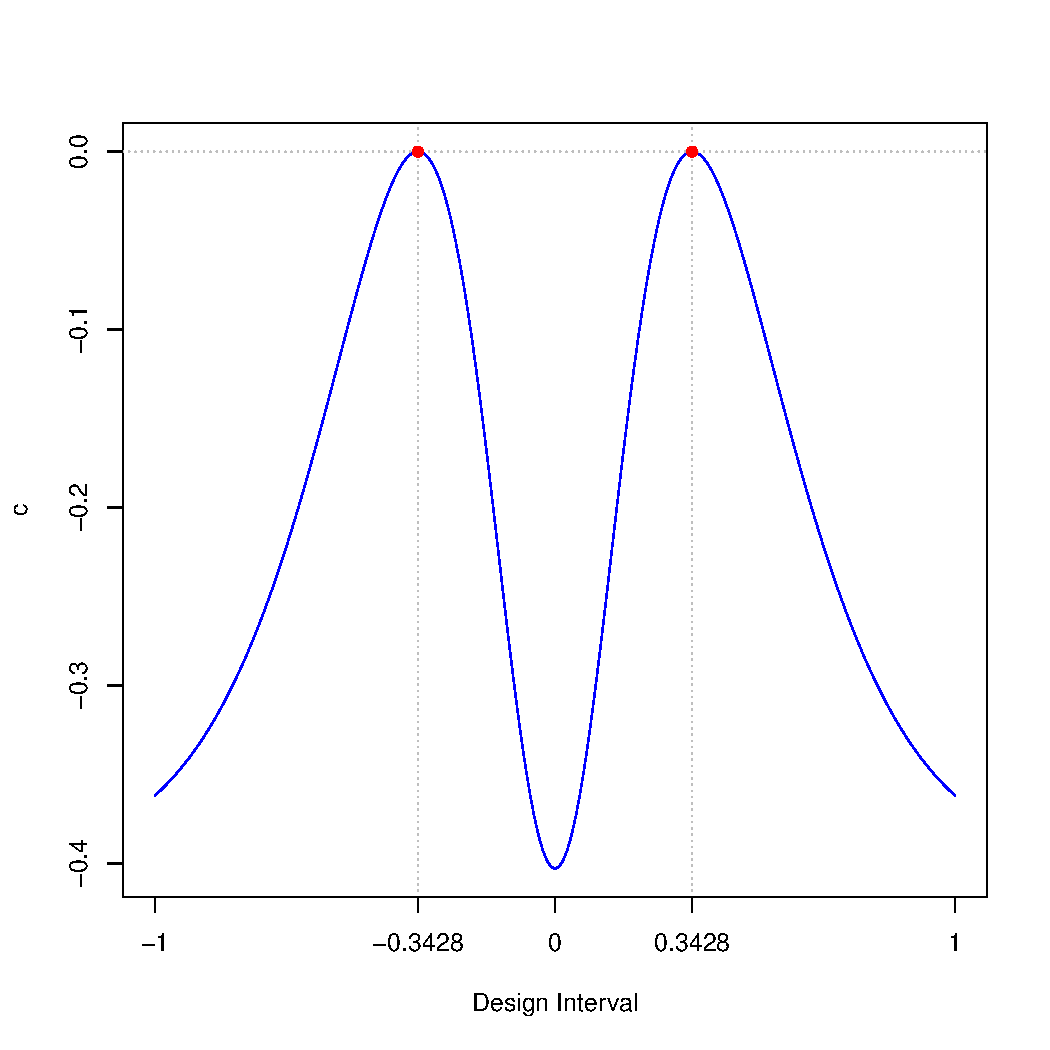
\includegraphics[width=.5\textwidth]{twoPL1.pdf}
}
\subfloat[][\code{Output from plot(twoPL2)}]{
  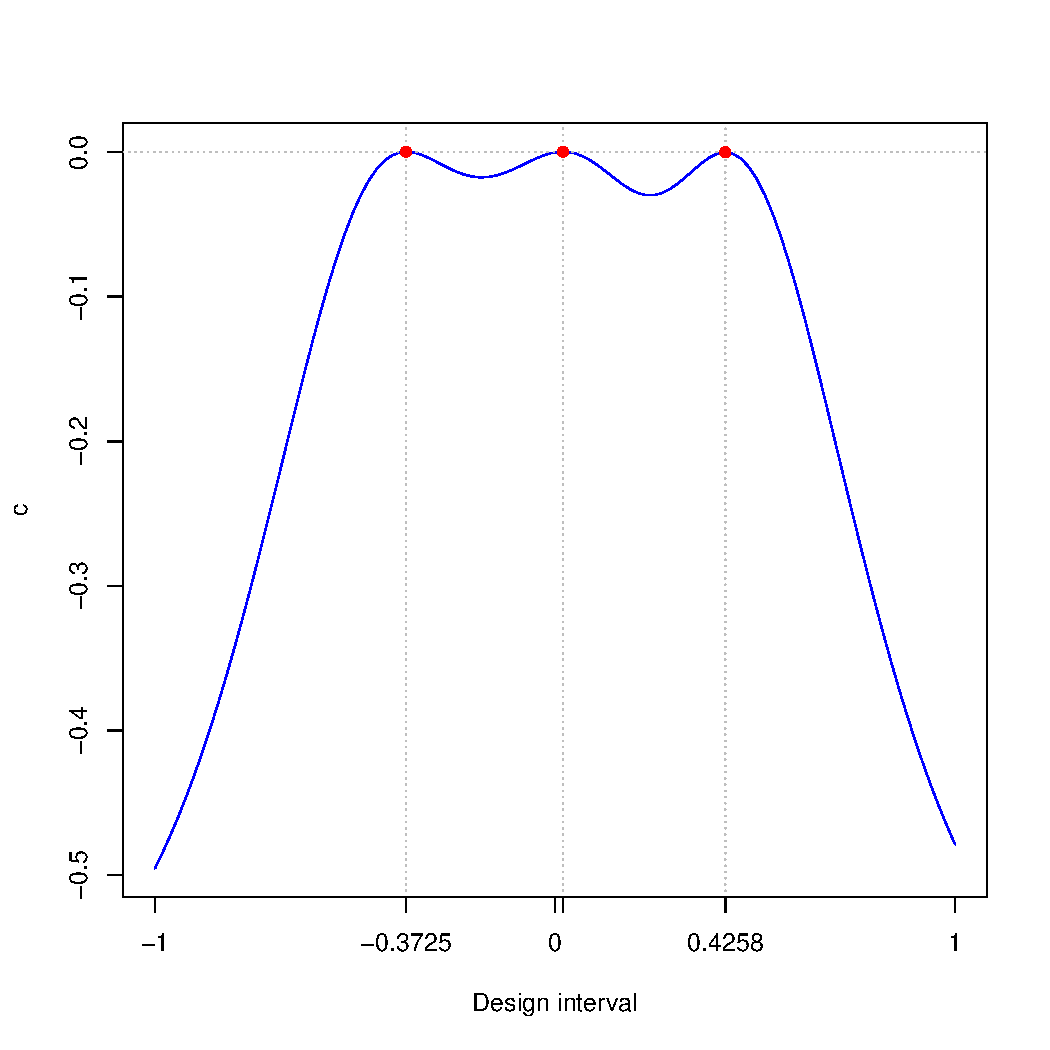
\includegraphics[width=.5\textwidth]{twoPL2.pdf}
}
\caption{
  Plots of the sensitivity functions of the generated $c-$optimal designs for estimating the ED95 when  $x \in \chi =  [-1, 1]$. The left panel (a) displays the sensitivity function of the locally  $c-$optimal design when $\btheta = (0, 7)$. The right panel (b) displays the sensitivity function of the  Bayesian $c-$optimal design  when $a\sim U(-0.3, 0.3)$ and $b \sim U(6, 8)$. Both (a) and (b) verify the optimality of the obtained designs. The solid red dots are the values of the sensitivity function at the obtained design points.
}
\label{fig:c-optimal-2pl}
\end{figure*}
%%%%%%%%%%%%%%%%%%%%%%%%%%%%%%%%%%%%%%%%%%%%%%%%%%%

Finding Bayesian $c-$optimal design is  very similar, except that each of~\eqref{eq:c-criterion} and \eqref{eq:c-criterion-sensitivity}	 must be  a vectorized R \code{function} with respect to the model parameters \code{a} and \code{b}:
  %with respect to the model parameters \code{a} and \code{b}:
  \begin{example}
R> c_opt_vec <-function(x, w, a, b, fimfunc){
+   gam <- log(.95/(1-.95))
+   M <- fimfunc(x = x, w = w, a = a, b = b)
+   B <- sapply(1:length(M), FUN = function(i)
+     matrix(c(1, -gam * b[i]^(-2)), ncol= 1) %*%
+       matrix(c(1, -gam * b[i]^(-2)), nrow = 1), simplify = FALSE)
+   sapply(1:length(M), FUN = function(i)
+     sum(diag(B[[i]] %*% solve(M[[i]]))))
+ }
R> c_sens_vec <- function(xi_x, x, w, a, b, fimfunc){
+   gam <- log(.95/(1-.95)) # LD .95
+   M <- fimfunc(x = x, w = w, a = a, b = b)
+   M_inv <- lapply(M , FUN = function(FIM) solve(FIM))
+   M_x <- fimfunc(x = xi_x, w = 1, a = a, b = b)
+   B <- sapply(1:length(M), FUN = function(i)
+     matrix(c(1, -gam * b[i]^(-2)), ncol= 1) %*%
+       matrix(c(1, -gam * b[i]^(-2)), nrow = 1), simplify = FALSE)
+   sapply(1:length(M), FUN = function(i)
+     sum(diag(B[[i]] %*% M_inv[[i]] %*% M_x[[i]] %*% M_inv[[i]])) -
+       sum(diag(B[[i]] %*% M_inv[[i]])))
+ }
\end{example}
In the \code{c\_opt\_vec} and \code{c\_sens\_vec}  functions, the arguments \code{a} and \code{b} are now vectors of the same (dynamic) length, and \fct{fimfunc} now returns a \code{list} of matrices  with length equal to \code{length(a)}.
Let $a\sim U(-0.3, 0.3)$ and $b \sim U(6, 8)$.
Given  \code{c\_opt\_vec} and \code{c\_sens\_vec}, the Bayesian $c-$optimal design for estimating the ED95  is obtained by
\begin{example}
R> twoPL2 <- bayes(formula = ~1/(1 + exp(-b * (x-a))), predvars = "x",
+                 parvars = c("a", "b"), family = "binomial",
+                 lx = -1, ux = 1,
+                 prior = uniform(lower = c(-.3, 6), upper  = c(.3, 8)),
+                 iter = 100, k = 3,
+                 crtfunc = c_opt_vec,
+                 sensfunc = c_sens_vec,
+                 ICA.control = list(rseed = 1, ncount = 60, checkfreq = Inf),
+                 sens.bayes.control = list(cubature = list(maxEval = 100)))
R> print(twoPL2)
Finding  Bayesian optimal designs

Call:
  ~1/(1 + exp(-b * (x - a)))

iter           x1         x2        x3         w1        w2        w3
1      1 -0.004009039 0.29828119 0.4605856 0.19080601 0.3821834 0.4270106
12    12  0.004988270 0.40974945 0.4383355 0.20244712 0.2165999 0.5809529
23    23 -0.353135960 0.03376940 0.4250446 0.04238018 0.2424870 0.7151328
34    34 -0.351030679 0.03608485 0.4284948 0.04107568 0.2404412 0.7184831
45    45 -0.370795161 0.02795782 0.4282277 0.03956796 0.2269339 0.7334982
56    56 -0.326444221 0.02699155 0.4266908 0.02763386 0.2197316 0.7526345
67    67 -0.359979100 0.02467998 0.4271671 0.02883547 0.2165489 0.7546157
78    78 -0.374296800 0.02160651 0.4265674 0.02691817 0.2180796 0.7550023
89    89 -0.372327659 0.01982217 0.4257716 0.02629106 0.2186265 0.7550825
100  100 -0.372518847 0.02002258 0.4257626 0.02640997 0.2186892 0.7549009
min_cost mean_cost
1   0.6555717 0.7701302
12  0.6288037 0.6371994
23  0.6267816 0.6297125
34  0.6265897 0.6281724
45  0.6258766 0.6279520
56  0.6254187 0.6278212
67  0.6253270 0.6277844
78  0.6252741 0.6277719
89  0.6252610 0.6277691
100 0.6252608 0.6277691

Optimal designs (k=3):
  Points1  Points2  Points3
-0.37252 0.02002  0.42576
Weights1 Weights2 Weights3
0.026    0.219    0.755

ICA iteration: 100
Criterion value:  0.6252608
Total number of function evaluations: 38461
Total number of successful local search moves: 1087
Total number of successful revolution moves: 134
Convergence: maxiter
Total number of successful assimilation moves: 1115
CPU time: 203.82  seconds!
  
  Maximum of the sensitivity function is  0.0003369562
Efficiency lower bound (ELB) is  0.9998316
Verification required 3.56 seconds!
  Adjust the control parameters in 'sens.minimax.control' ('n_seg')
or in 'sens.bayes.control' for higher speed.
R> twoPL2$design
iter         x1         x2        x3         w1        w2        w3  min_cost
1  100 -0.3725188 0.02002258 0.4257626 0.02640997 0.2186892 0.7549009 0.6252608
mean_cost     max_sens       elb time_sec
1 0.6277691 0.0003369562 0.9998316     3.56
\end{example}


Figure \ref{fig:c-optimal-2pl} (b) displays the plot of the sensitivity function of the design provided by the output  and it verifies its optimality.
Similar to the locally  $c-$optimal design, this design puts more than  $97\%$  of its weight on the positive support points.
\section{Summary}
\label{sec:summary}

\CRANpkg{ICAOD} modifies a state-of-the-art metaheuristic algorithm called Imperialist Competitive Algorithm   to find  different types of optimal designs for nonlinear models. We believe this package is more self-contained and has more capability than the few available in the literature. In particular, \CRANpkg{ICAOD} offers different design approaches  for handling the parameter dependency in the information matrix when the model is nonlinear. A useful feature of the \CRANpkg{ICAOD}  package is that it can  create  the Fisher information matrices for a very general class of  nonlinear models automatically and also includes useful theory-based tools   to assess proximity of any design to the   optimal design without knowing the latter.
Using \CRANpkg{ICAOD}, it is also possible  to find optimal designs for a user-specified optimality criterion, including hard-to-find various types of minimax   optimal designs for which the criterion is not differentiable.

Due to space consideration, we presented only a few   examples in this paper to   show the functionality of the package.
The help-documentation manual for the package contains further details and illustrations.  We hope that the generality and simplicity of the \CRANpkg{ICAOD} package will encourage researchers from different disciplines  to explore  optimal design ideas in their work and enable them to implement a more informed design to realize maximum statistical efficiency at minimal cost.


\section*{Computational details}
The results in this paper were obtained using
R~  4.0.2  with the
\CRANpkg{ICAOD}~ 1.0.1 package. R itself
and all packages used are available from the Comprehensive
R Archive Network (CRAN) at
\url{https://CRAN.R-project.org/}.


\section*{Acknowledgments}
We would like to thank Dr. Paul-Christian B\"urkner for his  helpful comments when writing the package and this manuscript.
The research of Wong reported in this paper was partially supported by a grant award R01GM107639 from the National Institute of General Medical Sciences of the National Institutes of Health.
The research of Holling and Masoudi  in this paper was partially supported by a grant (HO 1286/6 - 4) of the German Research Foundation (DFG).
The research of Kim reported in this paper was partially supported by grant awards R21GM140352 from the National Institute of General Medical Sciences and P30CA022453 from the National Cancer Institute of the National Institutes of Health.
The contents in this paper are solely the responsibility of the authors and do not necessarily represent the official views of the National Institutes of Health.

\section*{Disclosure}
Ehsan Masoudi is an employee of Roche Pharma AG in Germany since October 2019.

%\bibliography{ICAODV1}
\bibliography{masoudi-holling-wong-kim}

\address{Ehsan Masoudi\\
      Department of Psychology, University of M{\"u}nster\\
      Fliednerstr. 21, 48149 Germany\\
      \email{esn\_mud@yahoo.com}}

\address{Heinz Holling\\
    Department of Psychology, University of M{\"u}nster\\
    Fliednerstr. 21, 48149 Germany \\
  \email{holling@uni-muenster.de}}
  
\address{Weng Kee Wong\\
    Department of Biostatistics \\
    UCLA Fielding School of Public Health\\
    Los Angeles, CA 90095-1772, USA \\
    \email{wkwong@ucla.edu}}
    
\address{Seongho Kim\\
    Biostatistics and Bioinformatics Core, Karmanos Cancer Institute\\
    Department of Oncology, Wayne State University School of Medicine\\
    Detroit, MI 48201, USA \\
    \email{kimse@karmanos.org}}


\end{article}

\end{document}
